\onehalfspacing

\chapter{Comparison with known literature}

\label{chap:Chapter_5}

Until now we elaborated on the development of the numerical algorithm for the effective droplet model.
This model is built from the thin-interface approximation of the continuous model \Eqref{eqn:CHActive} and evolves the dynamics of the droplets via \Eqsref{eqn:DropletDiscretized} and dynamics of the background field $\phiOut$ using \Eqref{eqn:RD_dilute}.
We then laid out a procedure for choosing the optimum values for the various simulation parameters $\dx, \ell, \ds$ by comparing simulations of a test-case with the ground-truth i.e simulations using the continuous model.
We then arrived at the conclusion that $\dx \approx \ell \approx \ds$ is indeed an optimum choice for the simulation parameters, and finally the time-step $\dt$ is chosen from \Eqref{eqn:time_step} using the optimum values for $[\dx, \ell, \ds]$. 

We now demonstrate that the effective droplet model accurately captures the dynamics of the droplets and the background field in diverse scenarios, using the optimum values for the simulation parameters.
In Chapter \ref{chap:Introduction}, we discussed how biological cells use a setup featuring external chemical gradients and chemical reactions to control the position of droplets in their interior.
We cite a few more examples to put the point across. 

Rai et al. \cite{Rai2018} showed that during mitosis, an enzyme known as DYRK3 dissolves only selected condensates but keeps others such as P-bodies and nucleoli untouched, to prevent aberrant condensation.
The same kinase (DYRK3) is also known to dissolve stress granules during stress recovery, as shown by Wippich et al. \cite{Wippich2013}.
Brangwynne et al. \cite{Brangwynne2009} in their seminal work showed that P-granules localize to the posterior side in early stage \textit{C. elegans} embryos, which is governed by a gradient of a protein known as MEX-5.
On similar lines, Griffin et al. \cite{Griffin2011} showed how phosphorylation and dephosphorylation reactions generate concentration gradients throughout the cytoplasm.
Weber et al. \cite{Weber2017} utilized theory and simulations to explore the influence of chemical gradients on phase separation, thus shedding insights into how cells utilize local concentration gradients to spatially organize biomolecular condensates in their cytoplasm.

However, the cell also has to spatially control the ripening of condensates and preventing them from aggregating together and forming bigger droplets, which can happen due to Brownian mediated coalescence or \textit{Ostwald-Ripening}; see Refs. \cite{Review2019,Weber2017}.
Brownian mediated coalescence requires droplets to be physically close to each other, where they merge into bigger droplets upon contact. 
On the other hand, \textit{Ostwald-Ripening} is governed by gradients of chemical potential arising between the droplets as a result of unequal equilibrium volume fractions, due to heterogeneity in their size.
Generally, the cytoplasm inside the cell can show visco-elastic properties; see Ref. \cite {Xie2022}, which might lead to a slow ripening of the condensates.
Weiss et al. \cite{Weiss2004} also demonstrated that condensates can be strongly influenced by the cytoskeleton, and anomalous diffusion can arise due to molecular crowding, thus adversely affecting larger condensates and in turn not affecting diffusion across smaller condensates as much.
Thus, in this thesis, we will focus on \textit{Ostwald-Ripening} and we will not consider Brownian mediated coalescence. 

In the following section, we demonstrate that the effective droplet model is able to simulate two mechanisms (out of many), which the cell potentially uses to regulate the dynamics of condensates - in particular, chemical reactions and external chemical gradients.
To help disentangle the individual roles of these two mechanisms and to study how they affect dynamics of phase separated droplets, we consider them separately: first in simulations of single droplet systems, and then simulations of many droplet systems. 

We start by considering a simple scenario of a single passive droplet growing when immersed in a supersaturated background field.
We compare droplet growth using the effective droplet model, simulations using the continuous model and analytical results.
We then slowly build up complexity by adding chemical reactions and chemical gradients and more droplets; comparing them with simulations using the continuous model (wherever computationally possible) and analytical predictions, eventually reaching the situation where we simulate the coarsening dynamics of hundreds of droplets using the effective droplet model, as the continuous model is computationally expensive to be simulated.

\section{Passive droplet in a large background field}
We start by considering the simplest case of a passive droplet immersed in a large background field $\phiOut$.
We immerse the droplet in an initial volume fraction $\phi_\infty$ much greater than it's equilibrium volume fraction $\phiEqOut$, so the droplet grows in time. 
We demonstrate that the effective droplet model captures the growth of the droplet accurately when compared with simulations using the continuous model and analytical predictions.

As the droplet experiences an isotropic environment, the fluxes $\jOut$ entering the droplet from the background field will be isotropic in all directions, and hence the droplet will only grow and not drift; see \Eqsref{eqn:DropletDiscretized}.
We next derive the volume fractions inside and outside the droplet $\phiIn,~\phiOut$ analytically, enabling us to calculate the material fluxes $\jIn,~\jOut$, leading to droplet growth.

\subsection{Volume fraction profile and material fluxes inside the droplet}
Owing to symmetry, we place a spherically symmetric co-ordinate system at the centre of the droplet with $r$ being the radial co-ordinate.
Since $\phiIn$ inside the droplet typically varies only a little, we use the thin-interface approximation; see \Eqsref{eqn:thin_interface_model}, of the continuous model to approximately arrive at the dynamical equation for $\phiIn$ as:

\begin{align} 
    \label{eqn:RD_droplet_passive}
    \frac{\partial \phiIn}{\partial t}
        \approx D_\mathrm{in} \nabla^2 \phiIn,
\end{align}
where $D_\mathrm{in}$ is the diffusivity inside the droplet.
We invoke the standard \textit{quasi-static approximation} and assume that the droplet radius changes on a timescale which is much slower than the transients in \Eqref{eqn:RD_droplet_passive}; see Ref. \cite{Review2019}.

We can then analytically solve for $\phiIn$ from the stationary state of \Eqref{eqn:RD_droplet_passive}, using the boundary conditions $\phiIn(R) = \phiEqIn$ and $\partial_r \phiIn (0) = 0$ and we thus obtain a constant volume fraction inside the droplet as $\phiIn(r) = \phiEqIn$.

\subsection{Volume fraction profile and material fluxes outside the droplet}

Similar to inside the droplet, the volume fraction inside in the background field $\phiOut$ also typically varies a little and is hence described from the thin-interface approximation; see \Eqsref{eqn:thin_interface_model}, as:

\begin{align} 
    \label{eqn:RD_dilute_passive}
    \frac{\partial \phiOut}{\partial t}
        \approx D_\mathrm{out} \nabla^2 \phiOut,
\end{align}
where $D_\mathrm{out}$ is the diffusivity outside the droplet.
We solve for $\phiOut$ from the stationary state of \Eqref{eqn:RD_dilute_passive} using the boundary conditions $\phi_\mathrm{out}(R) = \phiEq_\mathrm{out}$ and far from the droplet $\phi_\mathrm{out}(\infty) = \phi_\infty$.
We thus obtain the volume fraction profile outside the droplet as $\phiOut(r) = \phi_\infty + (\phiEqOut - \phi_\infty) (R/r)$ and solution thus reveals that $\phiOut$ will monotonically approach $\phi_\infty$. 

\subsection{Material flux balance and droplet growth rate}

Spatial gradients in $\phiIn$ and $\phiOut$ lead to local material fluxes outside the droplet as $\vec{j}_\mathrm{out} \cdot \vec{n} = [-D_\mathrm{out} {\boldsymbol{\nabla}} \phiOut (R)] \cdot \vec{n} = -D \left[ \phi_{\infty}/R  - \phiEqOut / R \right]$, and inside the droplet as $\vec{j}_\mathrm{in} \cdot \vec{n} = [-D_\mathrm{in} {\boldsymbol{\nabla}} \phiIn (R)] \cdot \vec{n} = 0$.
Note that, we typically assume same diffusivity $D$ inside and outside the droplets, i.e. $D_\mathrm{out} \approx D_\mathrm{in} = D$.
The interfacial speed $v_n$ is calculated from
\Eqref{eqn:InterfacialSpeed}, and we can calculate the droplet growth rate from \Eqref{eqn:DropletGrowth} as:
\begin{equation}
	\label{eqn:interfacefluxes_passive}
	\frac{\mathrm{d} R}{\mathrm{d} t} = \frac{1}{S} \int_{\Omega} v_n ~ \mathrm{d}A = D\left ( \frac{\phi_{\infty}}{R}  - \frac{\phiEqOut}{R} \right ),
\end{equation}
where $S$ is the surface area of the droplet, $\Omega$ is the droplet surface and $\mathrm{d} A$ is the area element on the droplet surface.
Note that the only solution for ${\mathrm{d} R}/{\mathrm{d} t} = 0$ from \Eqref{eqn:interfacefluxes_passive} is $R_{\ast}$ (as $\phiEqIn,~\phiEqOut$ depend on the droplet radius $R$; see \Eqsref{eqn:GibbsThompsonRelations}). Droplets smaller than the critical radius $R_{\ast}$, defined as the radius at which the equilibrium volume fraction of the droplet equals the local supersaturation, dissolve quickly and is hence an unstable radius.

Having calculated the droplet growth rate analytically, we validate our choices for the optimum simulation parameters for the effective droplet model by simulating a single passive droplet of radius $R_0 = 2w$ embedded in a large supersaturated background field of value $\phiOut(t = 0) = \phi_\infty = 0.1$.
The droplet grows over time by ingesting material from the surroundings, as $\phiEqOut < \phi_\infty$.

Exploiting the symmetry of the problem, the continuous model uses a spherically symmetric domain of size $r \in [0, 400 w]$ and the effective droplet model uses a 3 dimensional periodic domain of size $[-L, L]^3$ with $L = 322 w$ with optimum simulation parameters $(\dx \approx \ell \approx \ds \approx R_0)$. Fig. \ref{fig:passive_droplet} shows a good agreement with the analytical prediction from \Eqref{eqn:interfacefluxes_passive} and the continuous model.

\begin{figure}[tb]
\centering
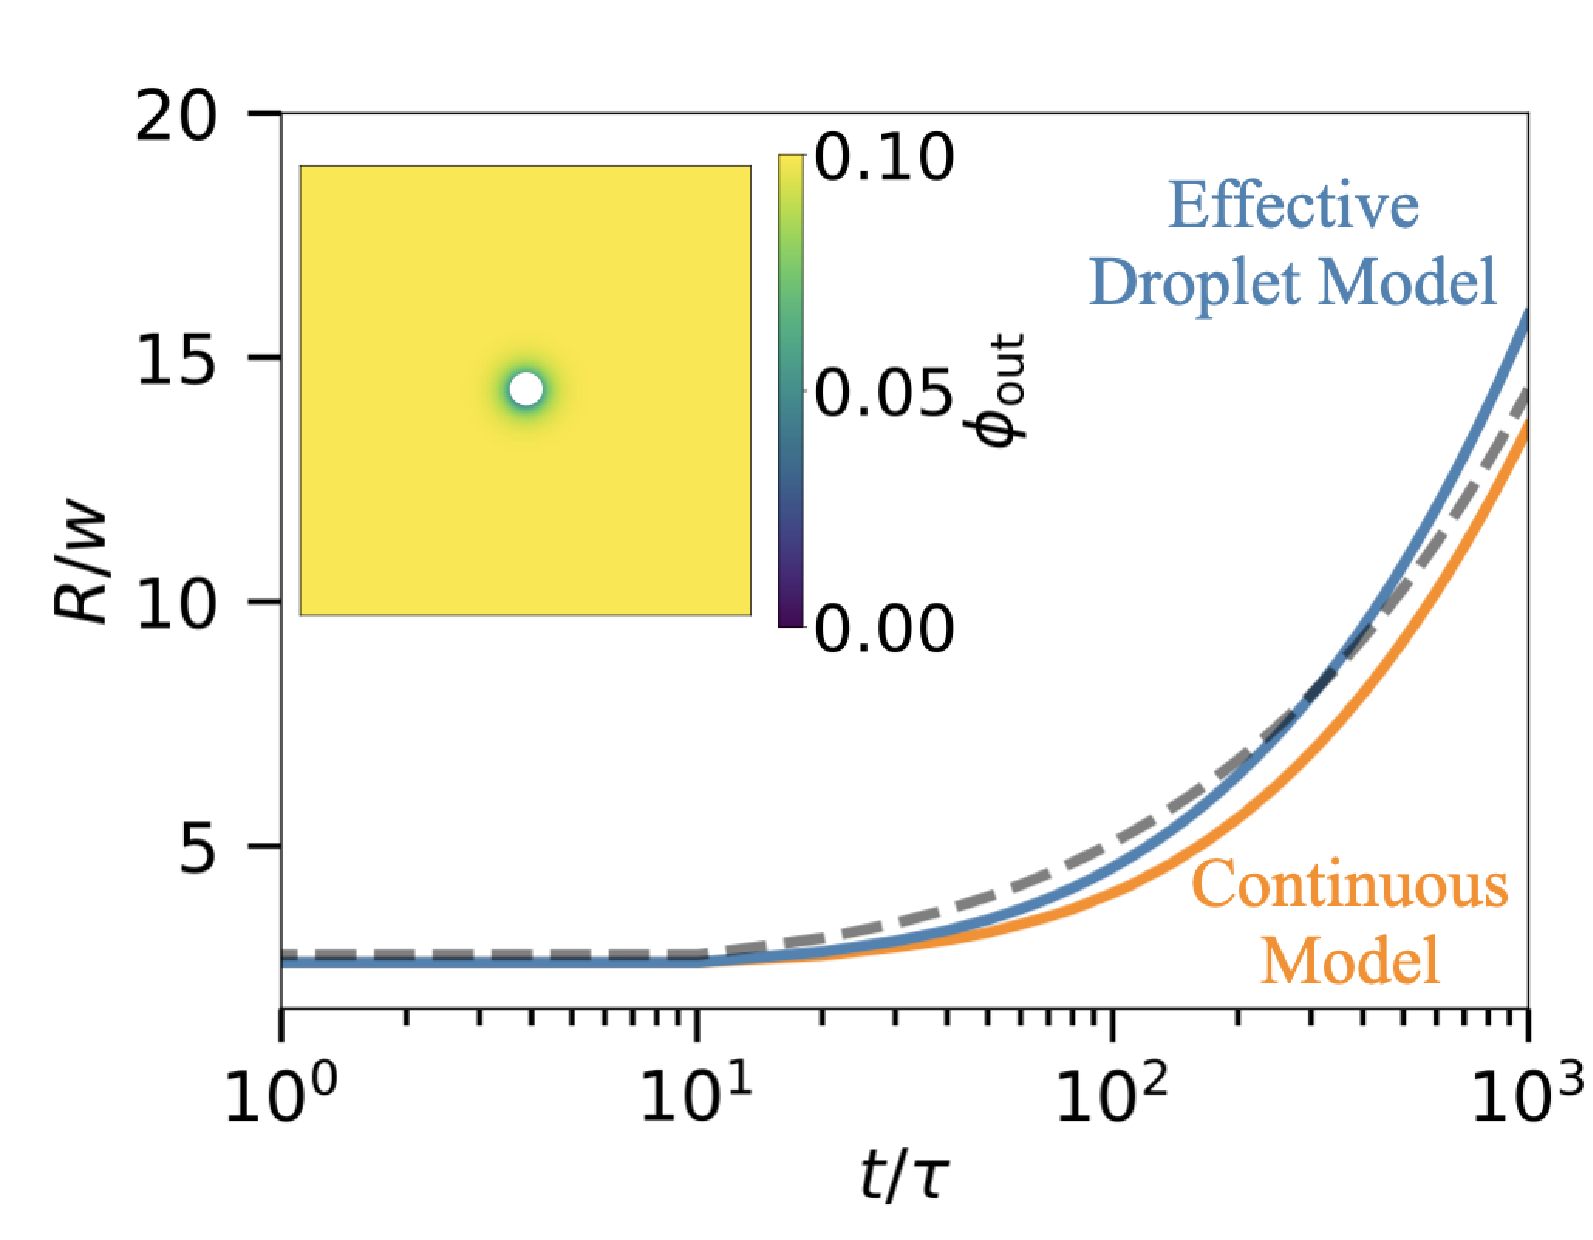
\includegraphics[scale=0.4]{MainContent/Figures/single_passive_droplet_growth.pdf}
\caption{
\textbf{Passive droplet growing when immersed a large supersaturated background field.}
Droplet radius $R$ as a function of time $t$ when immersed in a uniform supersaturation of volume fraction $\phi_\infty$.
Simulations using the effective droplet model with optimum parameters (blue line) matches well with analytical prediction from \Eqref{eqn:interfacefluxes_passive} (dashed line) and simulations using the continuous model (orange line).
Inset shows the simulation snapshot at $t = 10^3 \tau$ from the effective droplet model, with the droplet (in white) and the background field $\phiOut$ reaching $\phi_\infty = 0.1$ far from the droplet.
The continuous model uses a spherically symmetric domain with $r \in [0, 400 w]$ along with periodic boundary conditions and $\phi(\vec{r}, t=0) = \phi_\infty$.
The effective model uses a $3$-dimensional periodic domain of size $[-L, L]^3$ with $L = 322 w$, $\phiOut(\vec{r}, t=0) = \phi_\infty$, $\dx \approx \ell \approx \Delta s \approx R_0$ and periodic boundary conditions.
Remaining parameters are specified in Fig. \ref{fig:droplet_pair_schematics}.
}
\label{fig:passive_droplet}
\end{figure}

We next focus on a slightly complex situation where a passive droplet is immersed in a gradient of the droplet material.
Note that in this case, the droplet experiences a local a non-isotropic environment and may potentially drift in space.

\section{Passive droplet in an external volume fraction gradient}

Earlier studies by Weber et al. \cite{Review2019,Weber2017} have considered two-component phase separation with the inclusion of a third (inert) component called the regulator, which maintains an external gradient of the equilibrium volume fraction throughout the system.
Since we focus on a binary system, we impose a volume fraction gradient of the droplet material via appropriate boundary conditions.
Similar to the previous case of passive droplet, we again derive analytical predictions for the growth and drift of such a droplet using the thin-interface approximation and compare them with simulations performed using the continuous model and with the effective droplet model using the optimum parameters. 
We will first derive $\phiIn,~\phiOut$, enabling us to calculate the material fluxes $\jIn,~\jOut$, enabling us to predict droplet growth and drift.
Consider an isolated passive droplet of radius $R$ with a spherical co-ordinate system centred at the droplet position $\vec{x_0}$. 
The volume fraction outside the droplet can thus be expressed as $\phiOut(r, \theta, \varphi)$, where $r$ is the radial distance from the centre of the droplet and $\theta \in [0, 2 \pi), \varphi \in [0, \pi]$ are the polar and azimuthal angles.
Without loss of generality, we assume that the droplet experiences a one dimensional gradient that varies along the $x$-coordinate as seen from \figref{fig:drop_in_gradient_schematic}.

In general, a position dependant supersaturation outside the droplet might lead to non-spherical droplets and possible deformations in their shapes. 
However, in this thesis, we focus solely on spherical droplets by assuming that a large surface tension $\gamma$ quickly nullifies any deformations in droplet shape.

Contrary to the case of a passive droplet in a supersaturated medium, the droplet here experiences a volume fraction $\phi_{\infty}$, which far from the droplet reads as $\phi_{\infty} = \alpha + \beta \, r \, \text{cos}\,\varphi$ because of the existence of the external gradient; see \figref{fig:drop_in_gradient_schematic}.
Here $\alpha, \beta$ are the mean volume fraction and strength of the gradient respectively at the position of the droplet. 

\begin{figure}[tb]
\centering
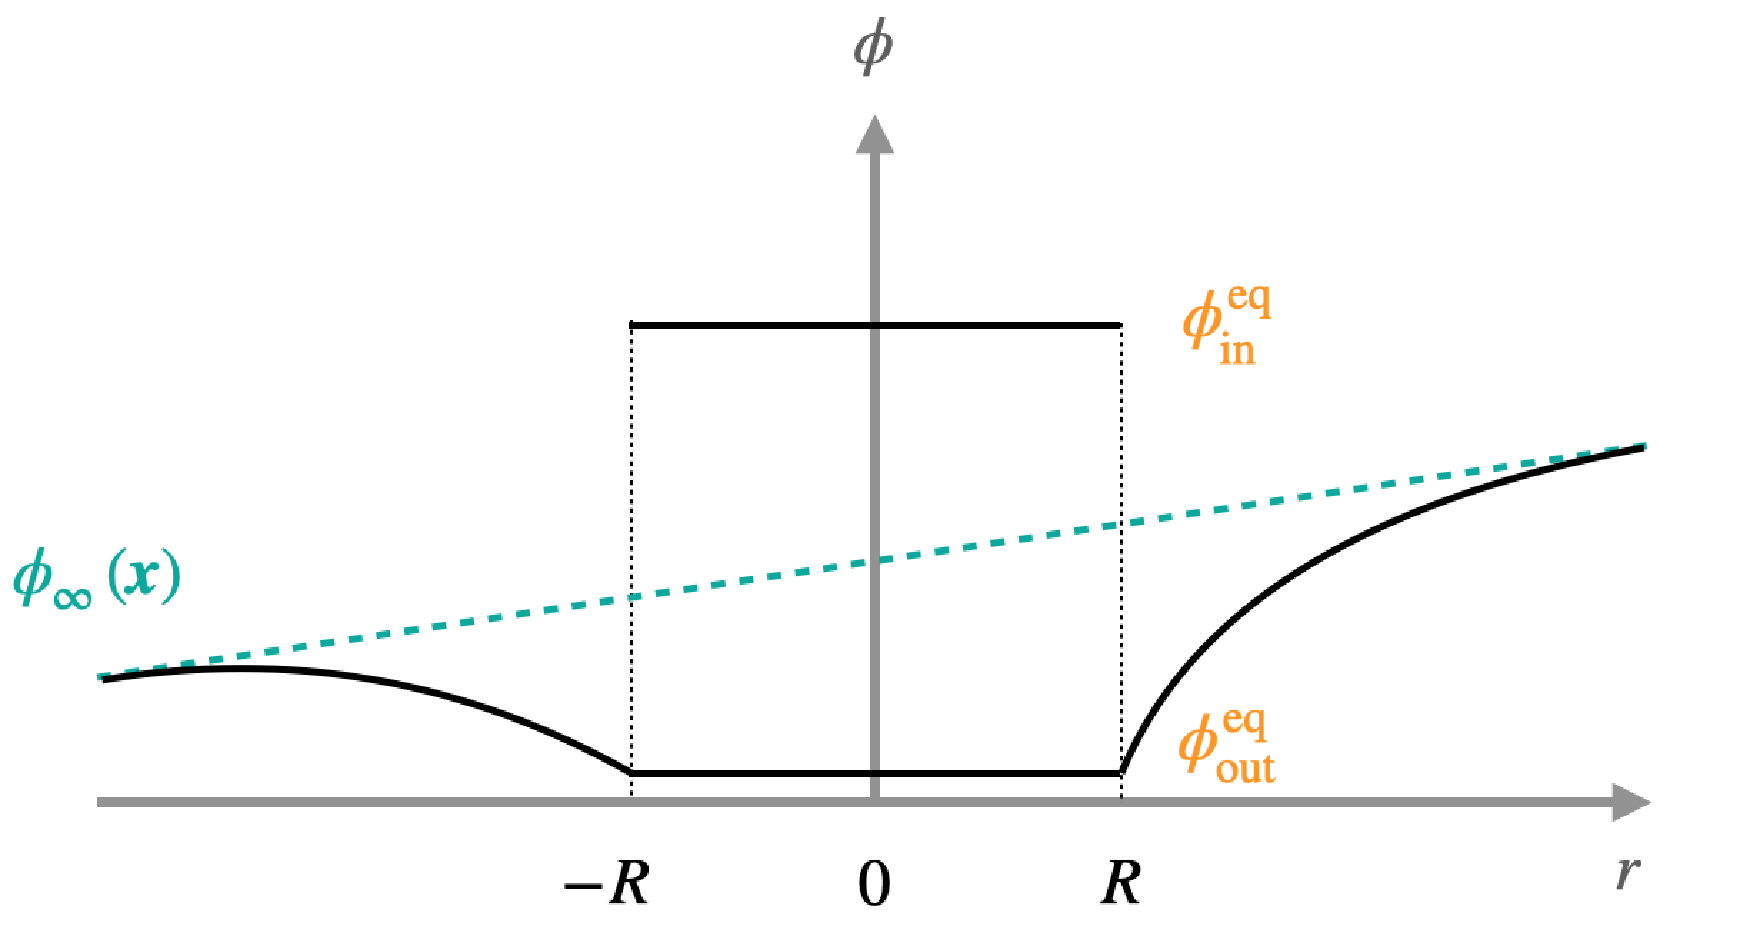
\includegraphics[scale=0.4]{MainContent/Figures/drop_in_gradient_schematic.pdf}
\caption{\textbf{Schematics of volume fractions inside and outside of a passive droplet immersed in an external volume fraction gradient.}
A droplet of radius $R$ at location $\vec{x} = 0$ is placed in a position dependant volume fraction $\phi_\infty (\vec{x})$.
$\phiEqIn,~\phiEqOut$ are volume fractions inside and outside the interface, given by \Eqsref{eqn:GibbsThompsonRelations}.
}
\label{fig:drop_in_gradient_schematic}
\end{figure}

We invoke the thin-interface approximation; see \Eqsref{eqn:thin_interface_model}, and as $\phiIn$ inside the droplet typically varies only a little, we solve for $\phiIn$ from the steady state of \Eqref{eqn:RD_droplet_passive}, using the boundary conditions $\phiIn(R) = \phiEqIn$ and $\partial_r \phiIn (0) = 0$ to obtain $\phiIn(r) = \phiEqIn$.
Similar to inside the droplet, the volume fraction inside in the background field $\phiOut$ also typically varies a little; see \Eqsref{eqn:thin_interface_model}, and can be solved from \Eqref{eqn:RD_droplet_passive} using the boundary conditions $\phi_\mathrm{out}(R) = \phiEq_\mathrm{out}$ and far from the droplet $\phi_\mathrm{out}(\infty) = \phi_{\infty} = \alpha + \beta \, r \, \text{cos}\,\varphi$.
We thus obtain the volume fraction profile outside the droplet as:
\begin{equation*}
    \phiOut(r, \varphi) = \alpha \left ( 1 - \frac{R}{r} \right ) + \beta \, \text{cos} \varphi \left ( r - \frac{R^3}{r^2} \right ) + \phiEqOut\,\frac{R}{r}.
\end{equation*}
We evaluate the local fluxes at the droplet surface as:
\begin{subequations}
\begin{align}
    \jIn \cdot \vec{n} &= [-D {\boldsymbol{\nabla}} \phiIn (R)] \cdot \vec{n} = 0 \mathrm{~and~} \nonumber
    \\[10pt]
    \jOut \cdot \vec{n} &= [-D {\boldsymbol{\nabla}} \phiOut (R)] \cdot \vec{n} = -D \left ( 3 \beta \text{cos} \varphi  + \frac{\alpha}{R} - \frac{\phiEqOut}{R} \right ), \nonumber
\end{align}
\end{subequations}
where we assume equal diffusivities inside and outside the droplet.
Note that $\jOut \cdot \vec{n}$ has an angular dependence, and hence the droplet will drift as a result of unequal fluxes on it's surface.
We then calculate the interfacial speed $v_n$ from \Eqref{eqn:InterfacialSpeed} and arrive at the droplet growth and drift speed along the $x$ co-ordinate from \Eqref{eqn:DropletGrowth} and \Eqref{eqn:DropletDrift} as:

\begin{subequations}
\label{eqn:interfacefluxes_gradient}
\begin{align}
	\frac{\mathrm{d} R}{\mathrm{d} t} &= \frac{1}{4 \pi} \int_{\Omega} D \left ( 3\,\beta \, \text{cos} \, \varphi  + \frac{\alpha}{R} - \frac{\phiEqOut}{R} \right ) \mathrm{d}A = \frac{D\,\alpha}{R} - \frac{D \phiEqOut }{R}
	\text{~and}
\\[10pt]
    \frac{\mathrm{d} x_0}{\mathrm{d} t} &= \frac{3}{4 \pi} \int_{\Omega} D \left ( 3\,\beta \, \text{cos} \, \varphi  + \frac{\alpha}{R} - \frac{\phiEqOut}{R} \right ) \text{cos} \, \varphi \, \mathrm{d}A = 3 D \beta,
\end{align}
\end{subequations}
where $\Omega$ is the droplet surface and $\mathrm{d} A$ is the area element on the droplet surface. 
Note that the drift speed is a constant value depending only on the strength of the gradient $\beta$ and the diffusivity $D$.
Naturally, increasing $\beta$ would lead to higher drift speeds for a constant diffusivity.

Having calculated the droplet growth rate and drift speed  analytically, we validate our choices for optimum parameters for the effective droplet model. 
We simulate a single passive droplet of initial radius $R_0 = 20w$ immersed in a linear volume fraction gradient of the droplet material maintained via appropriate boundary conditions. 
Similar to the case of the passive droplet growing in a supersaturated medium, the passive droplet in this case also grows over time by taking material from the surroundings. 
Furthermore, as $\jOut \cdot \vec{n}$ has a angular dependence, it results in unequal fluxes leading to droplet drift along the gradient.

Depending on the strength of the gradient $\beta$, we demonstrate that the effective droplet model captures droplet dynamics in both situations - for high and low value of $\beta$.
We first consider the case of high $\beta = 8.3 \times 10^{-5} w^{-1}$, as shown in Fig. \ref{fig:drop_in_gradient}A and Fig. \ref{fig:drop_in_gradient}B.
The continuous model uses a cylindrical domain with $r \in [0, 400 w]$, $z\in [-L_1, L_1]$ with $L_1=600 w$, azimuthal symmetry, and boundary conditions $\mu(z=-L_1) = 0$ and $\mu(z=L_1)= 0.072\,b w^3$ to impose the gradient.
Note that imposing a condition on the chemical potential $\mu$ means that the system can be assumed to be coupled to infinite reservoirs at it's $z$-boundaries, which enables us to maintain the gradient of the volume fraction field $\phi$ throughout the system. 
The effective model uses a $3$-dimensional box of size $[-L_2, L_2]^3$ with $L_2 = 422 w$, $\dx \approx \ell \approx \Delta s \approx R_0$, and boundary conditions $\phiOut(y = -L_2) = 0.01483$ and $\phiOut(y = L_2) = 0.0851$.
Fig. \ref{fig:drop_in_gradient}B shows a good agreement with the analytical predictions for droplet growth and drift from \Eqsref{eqn:interfacefluxes_gradient} and simulations using the continuous model.
We then consider the scenario with low $\beta = 4.2 \times 10^{-5} w^{-1}$, as shown in Fig. \ref{fig:drop_in_gradient}C and Fig. \ref{fig:drop_in_gradient}D.
The continuous model for this case uses the same parameters as the case with high $\beta$, but with boundary conditions $\mu(z=-L_1) = 0$ and $\mu(z=L_1)= 0.0427\,b w^3$ to impose the gradient.
The effective model uses the same parameters as the case with high $\beta$, but with boundary conditions $\phiOut(y = -L_2) = 0.007$  and $\phiOut(y = L_2) =  0.042$.
Fig. \ref{fig:drop_in_gradient}D also shows a good agreement with the analytical predictions for droplet growth and drift from \Eqsref{eqn:interfacefluxes_gradient} and simulations using the continuous model.

Additionally, it is interesting to see that increasing approximations of the continuous model (in orange) lead to increasingly worse estimates for droplet drift, as the analytical predictions from the thin-interface approximation (dashed line); see \Eqsref{eqn:thin_interface_model}, are approximations of the continuous model, and the effective droplet model (in blue) is an approximation of \Eqsref{eqn:thin_interface_model}.
Finally, note that the match for the droplet drift speed, given by $(\mathrm{d} x_0 / \mathrm{d} t = 3 D \beta)$ in three dimensions, gets worse for increasing $\beta$, which is expected, as seen from Fig. \ref{fig:drop_in_gradient}B and Fig. \ref{fig:drop_in_gradient}D.

\clearpage

\begin{figure}[tb]
\centering
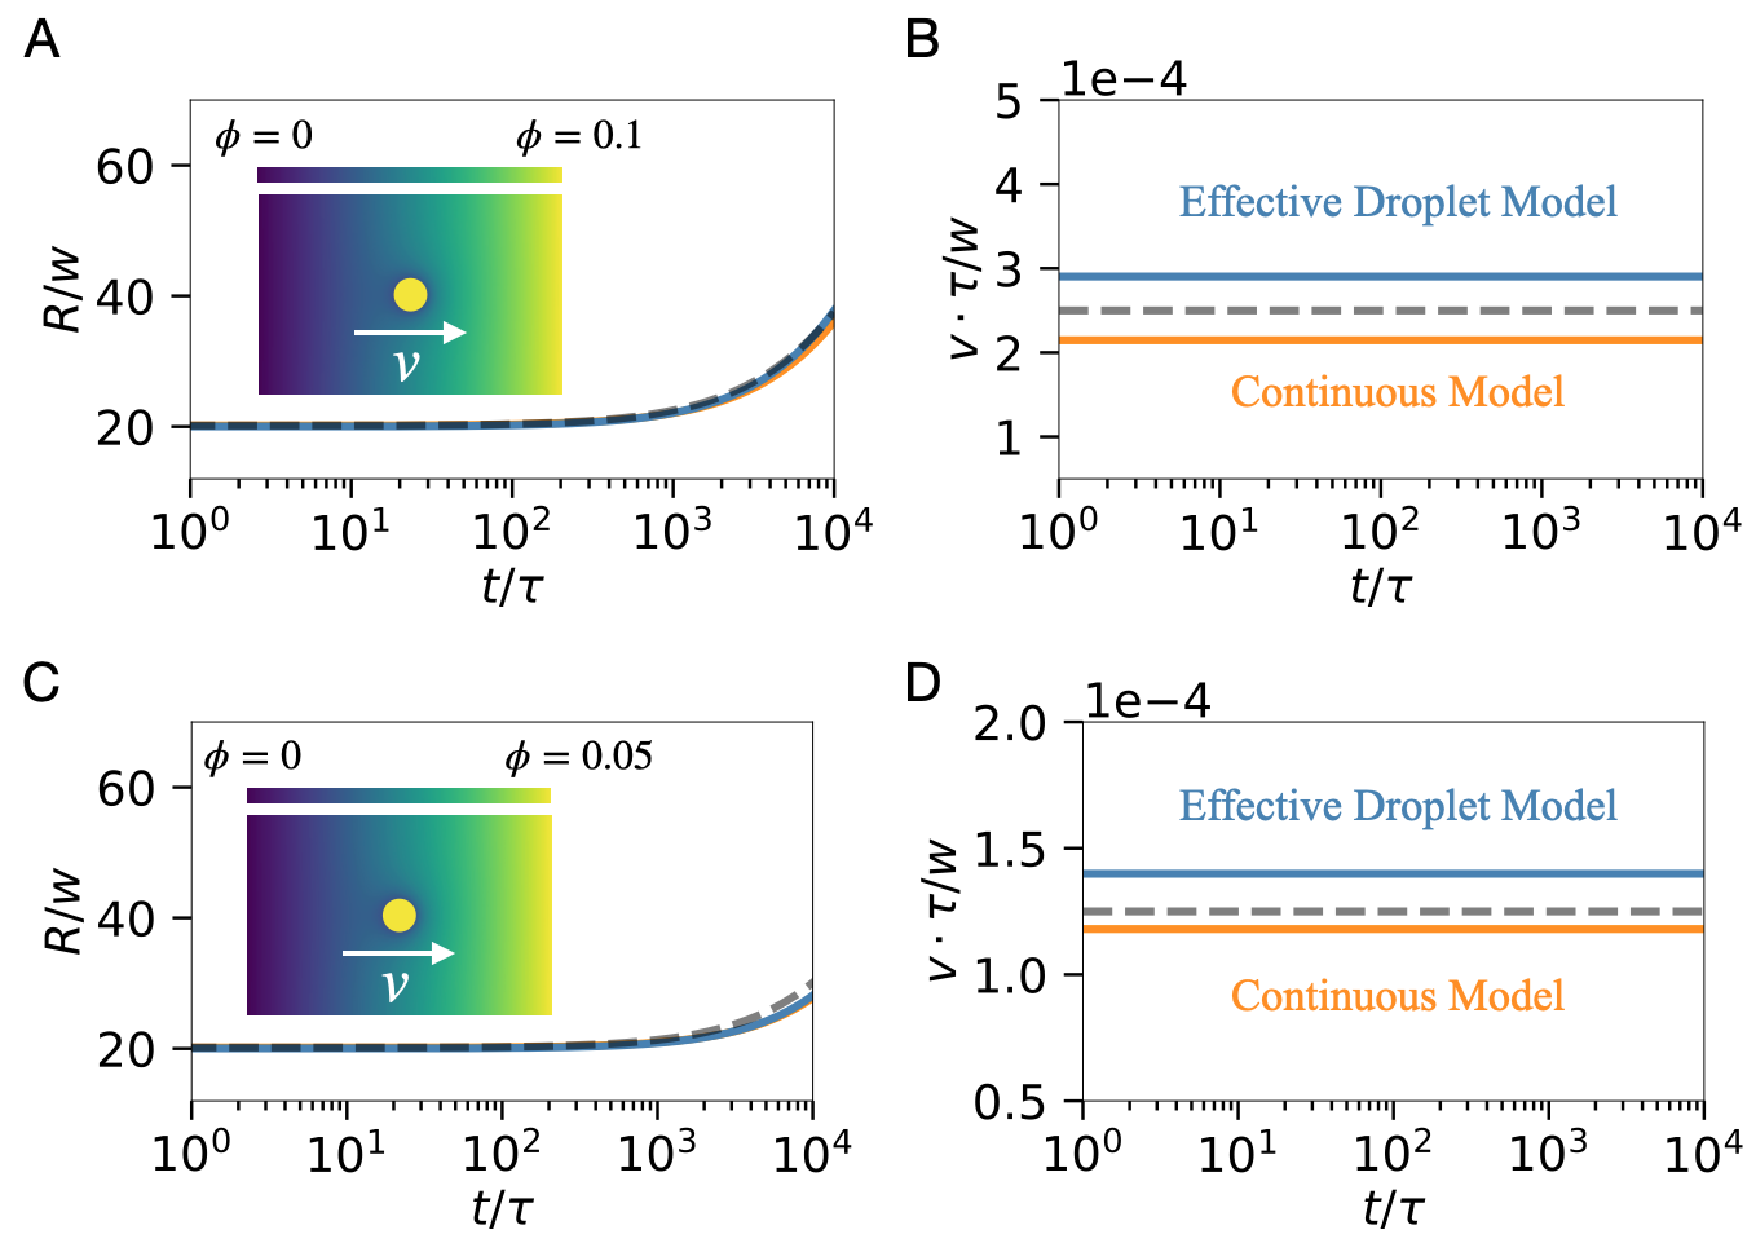
\includegraphics[scale=0.5]{MainContent/Figures/drop_in_gradient.pdf}
\caption{
\textbf{Droplet dynamics in external gradients.}
(A) Droplet radius $R$ as a function of time $t$ for the effective droplet model (blue), analytical prediction (dashed line) and the continuous model (orange).
The inset shows a schematic of the simulation with the strong gradient of droplet material imposed in the background.
(B) Droplet drift speed $v$ as function of $t$.
\mbox{(C, D)} Droplet radius $R$ and drift speed $v$ versus time $t$ for a weak gradient. 
\mbox{(A, B)}
The continuous model uses a cylindrical domain with $r \in [0, 400 w]$, $z\in [-L_1, L_1]$ with $L_1=600 w$ and azimuthal symmetry along with the boundary conditions $\mu(z=-L_1) = 0$ and $\mu(L_1)= 0.072\,b\,w^3$ to maintain the gradient throughout the system.
The effective model uses a $3$-dimensional box of size $[-L_2, L_2]^3$ with $L_2 = 422 w$, $\dx \approx R_0$, $\ell \approx \Delta s \approx R_0$ along with the boundary conditions $\phiOut(y = -L_2) = 0.01483$ and $\phiOut(y = L_2) = 0.0851$.
\mbox{(C, D)}
To maintain the gradient throughout the system, the continuous model uses the boundary conditions $\mu(z=-L_1) = 0$ and $\mu(z = L_1)= 0.0427\,b\,w^3$ and the effective droplet model uses the boundary conditions $\phiOut(y = -L_2) = 0.007$ and $\phiOut(y = L_2) = 0.042$ with the remaining parameters same as \mbox{(A, B)}.
Note that in the absence of droplets, boundary conditions imply identical linear gradient in the continuous model as $\phi = \phi(z)$ and in the effective droplet model as $\phiOut = \phiOut(y)$, which were also used to initialize the background for both the models.
Remaining parameters are specified in Fig. \ref{fig:droplet_pair_schematics}.
}
\label{fig:drop_in_gradient}
\end{figure}

\clearpage

\begin{figure}[tb]
\centering
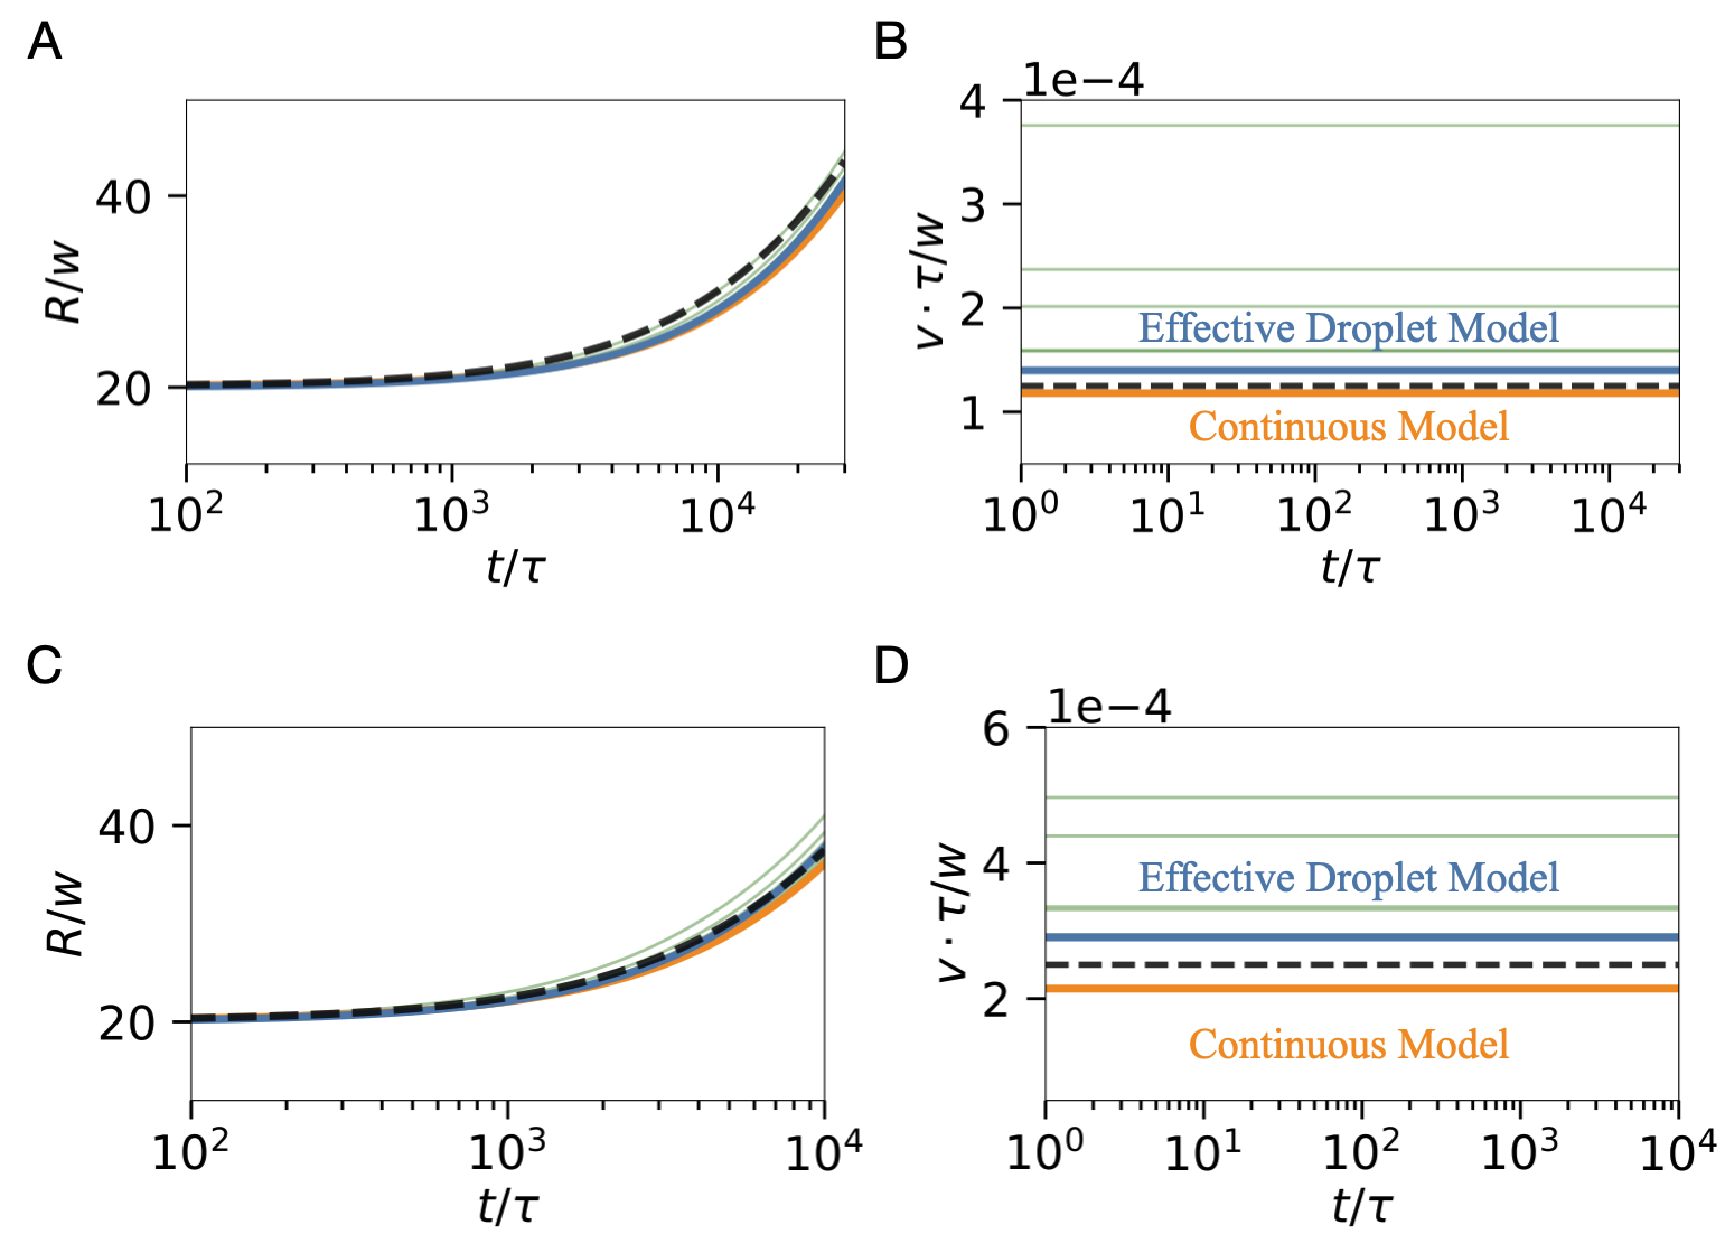
\includegraphics[scale=0.5]{MainContent/Figures/drop_in_gradient_all.pdf}
\caption{
\textbf{Effect of varying shell thickness $\ell$ on droplet dynamics in external gradients.}
(A, C) show droplet radius $R$ and (B, D) show drift speed $v$ as a function of time $t$ for continuous model (orange), the effective droplet model with optimum parameters $(\dx \approx \ell \approx \ds \approx R_0)$ (blue), the effective droplet model with varying shell thickness $\ell$ (green) and the analytical prediction (dashed line).
\mbox{(A, B)} Simulations performed for the same parameters as in \figref{fig:drop_in_gradient}A and \figref{fig:drop_in_gradient}B.
\mbox{(C, D)} Simulations performed for the same parameters as in \figref{fig:drop_in_gradient}C and \figref{fig:drop_in_gradient}D.
Droplet growth remains fairly unaffected, but droplet drift speed $v$ is highly sensitive to changes in $\ell$, with (B) and (D) highlighting the importance of choosing the optimum value for $\ell$.
Shell thickness values are uniformly chosen between $\ell \in [0.25 R_0, 10R_0]$ with $\dx \approx \ds \approx R_0$.
}
\label{fig:drop_in_gradient_all}
\end{figure}

Lastly, we study the accuracy of the effective droplet model for simulation parameters other than the optimum values.
We keep $\dx, \ds$ at their optimum value ($\dx \approx \ds \approx R_0$), but uniformly vary the shell thickness between $\ell \in [0.25 R_0, 10R_0]$.

Fig. \ref{fig:drop_in_gradient_all} reveals the importance of choosing the optimum value for $\ell$ and further validates our choice of the optimum simulation parameters.
For both the cases - high (Fig. \ref{fig:drop_in_gradient_all}A, Fig. \ref{fig:drop_in_gradient_all}B) and low (Fig. \ref{fig:drop_in_gradient_all}C, Fig. \ref{fig:drop_in_gradient_all}D) strength of the gradient $\beta$, the droplet growth remains unaffected but the drift speed $v$ is highly sensitive to the value of $\ell$.
Strong deviations from the droplet drift speed occur for values of $\ell$ which are either too small or too large compared to $\dx$.
As mentioned before, the flux $\jOut^{(m)} \cdot \vec{n}$ outside each droplet for each $m$-th shell sector scales with $\ell^{-1}$; see Appendix \ref{sec:fluxes_inside_shell}.
Thus small values of $\ell$ imply larger fluxes, implying a stronger droplet drift speed. 
For values of $\ell$ which are too large, the droplet drift speed again deviates strongly from the analytical prediction from \Eqsref{eqn:thin_interface_model}.
This is because for large $\ell$, the value of $\phiShell^{(m)}$ is higher than the true value (which is near the droplet) as a result of the gradient of $\phiOut$.
Thus, for large $\ell$, $\phiShell^{m}$ is calculated far away from the droplet, leading to an erroneous representation of $\phiOut$ close to the droplet.
Lastly, we also perform simulations for 2 dimensional systems; see Appendix \ref{sec:droplet_gradient_2D}, and validate our choice for the optimum simulation parameters. 

Taken together, the effective droplet model accurately captures the effects of external gradients on droplet dynamics, both in low and high values of the gradient and for two; see Appendix \ref{sec:droplet_gradient_2D}, and three dimensional systems. 
However, the difference in simulation times is stark between the continuous model ($\sim 10 \mathrm{~simulation~days}$) and the effective droplet model ($\sim 10 \mathrm{~simulation~minutes}$ with optimum parameters) with identical High-performance computing hardware for simulations in \figref{fig:drop_in_gradient} and \figref{fig:drop_in_gradient_all}, thus making the effective droplet model a computationally viable alternative to the continuous model when simulating such systems.

Next, we shift our attention to demonstrating the hallmark of this model - which is the ability to simulate large three dimensional systems with many droplets.
Note that again we do not simulate this scenario using the continuous model, as it is computationally expensive.
In this case, we compare the effective droplet model only with analytical predictions. 
We begin by discussing the interactions of many passive droplets in a dilute emulsion.

\section{\textit{Ostwald-Ripening} in passive emulsions}

In emulsions consisting of many passive droplets, large droplets typically grow at the expense of smaller droplets, a phenomenon known as \textit{Ostwald-Ripening}; see Refs. \cite{Review2019,LSWanalytics}.
Consider a system of $N$ passive droplets with radii $R_i$, which are far apart from each other. 
The droplets are immersed in a large background field of low supersaturation and hence, nucleation events are rare.
As the droplet density is small and the supersaturation is low, all the droplets share a common supersaturation $\phi_\infty (t)$, through which all droplet-droplet interactions are mediated.
Each droplet then behaves like an isolated droplet which experiences a volume fraction $\phi_\infty(t)$ far away from it, which depends on the number of droplets present and on time.
From volume conservation, the dynamics of the supersaturation $\phi_\infty$ is described as:
\begin{equation}
\label{eqn:LSW_theory}
    \overline{\phi}\,V_\mathrm{system} = \phiEqIn \, \sum_{i=1}^{N} V_i(t) + \phi_\infty(t) \left ( V_\mathrm{system} - \sum_{i=1}^{N} V_i(t) \right ),
\end{equation}
where $V_\mathrm{system}$ is the system volume, $V_i(t)$ is the volume of a single droplet of radius $R_i(t)$.
Thus, droplet dynamics is still determined by \Eqref{eqn:interfacefluxes_passive}, but the supersaturation each droplet encounters far from it is governed by \Eqref{eqn:LSW_theory}.

Assuming a large system as compared to the droplet volumes $V_\mathrm{system} \gg \sum_{i=1}^{N} V_i(t)$ and neglecting any spatial correlations between the droplets, Lifshitz and Slyozov predicted that the average droplet radius $\left \langle R_i \right \rangle$ grows as $t^{1/3}$ in this case; see Refs. \cite{Lifshitz,Wagner,LSWanalytics}.
In such dilute emulsions, large droplets grow at the expense of smaller droplets, in which the average droplet radius $\left \langle R \right \rangle$ in the system grows as $\left [ {\left \langle R_i \right \rangle} ^{3}(t) - {\left \langle R_i \right \rangle}_0^{3}(t) \right ] \propto t$, where ${\left \langle R_i \right \rangle}_0$ indicates the initial average radius of the droplets.

Furthermore, in the limit of vanishing supersaturation, \textit{Ostwald-Ripening} follows the \textit{Lifshitz-Slyozov-Wagner} scaling laws, where the re-scaled radius $\rho = R_i/{\left \langle R_i \right \rangle}$ follows a universal shape of the droplet-size distribution $H(\rho)$; see Refs. \cite{Review2019,LSWanalytics}, as:

\begin{equation}
\label{eqn:LSW_histogram}
    H(\rho) = \frac{4}{9} \, \rho^2\left ( 1+ \frac{\rho}{3} \right ) ^ {-7/3} \left ( 1-\frac{2 \rho}{3} \right )^{-11/3} \mathrm{exp} \left ( 1 - \frac{3}{3 - 2\rho} \right ).
\end{equation}
Having briefly described the analytical predictions for droplet growth and size distribution for a system of passive droplets undergoing \textit{Ostwald-Ripening}, we next demonstrate that our effective droplet model captures these predictions well. 

Indeed our simulation of $10^5$ droplets indeed recovers the $t^{1/3}$ scaling; see \figref{fig:passive_emulsions}A, when we simulate a dilute emulsion by setting the discretization $\dx$ to the system size (and thus $\ell \approx \dx$), as a mean-field approach is desired.
Note that we need a single sector to discretize the vicinity of each droplets, as they are assumed to be far from each other and thus their vicinity is nearly isotropic.
Moreover, \figref{fig:passive_emulsions}B shows that the distribution of radii also follows the universal shape $H(\rho)$ given by \Eqref{eqn:LSW_histogram}.
Our effective model thus faithfully captures the dynamics of many droplets, optionally even beyond the Lifshitz-Slyozov regime by increasing the spatial resolution to capture correlations in droplet growth.

\begin{figure}[tb]
\centering
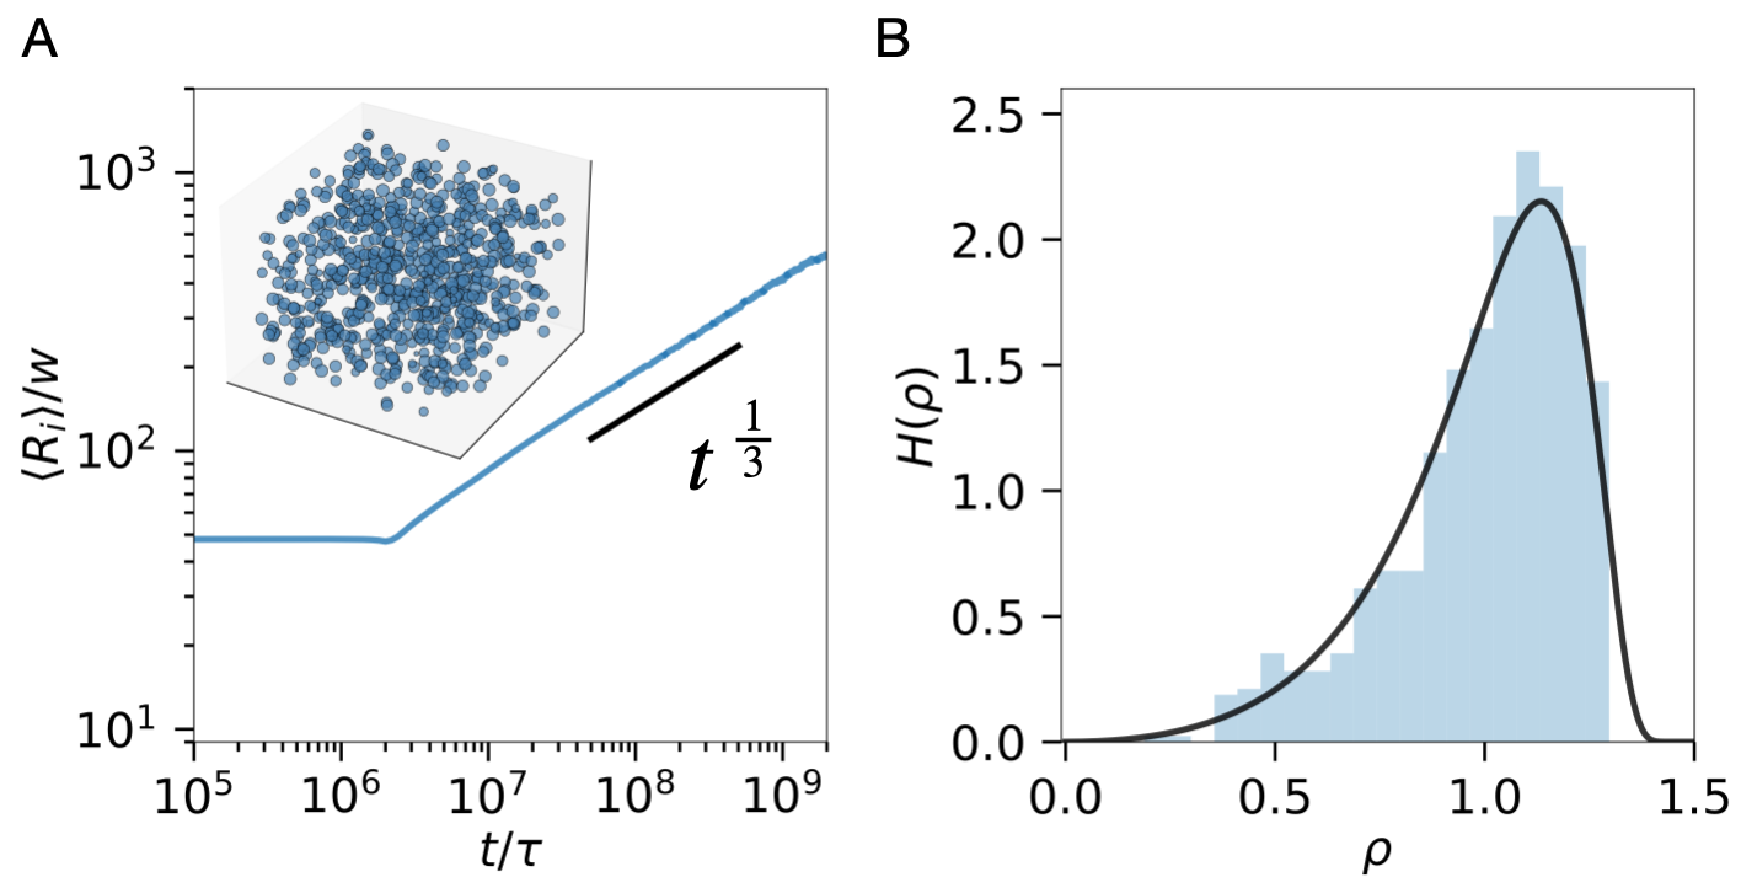
\includegraphics[scale=0.5]{MainContent/Figures/passive_emulsions.pdf}
\caption{\textbf{\textit{Ostwald-Ripening} in passive emulsions}.
(A) Mean droplet radius $\langle R_i \rangle$ as a function of time $t$ shows the expected scaling $\langle R_i \rangle \propto t^{1/3}$; see Refs. \cite{Lifshitz,Wagner,LSWanalytics}.
Inset shows snapshot at $t=2 \times 10^8 \tau$.
(B) Frequency $H(\rho)$ of the re-scaled mean radius $\rho = R_i/\left \langle R_i \right \rangle$ at $t = 2 \times 10^8 \tau$ compared to the expected universal distribution (black); see Refs. \cite{Lifshitz,Wagner}.
(A, B)
Simulations using the effective droplet model were carried out in a $3$ dimensional periodic cubic domain of size $[0, L]^3$, where $L = 10^4 w$.
We used $\Delta x \approx \ell \approx L$ and a single shell sector to approach the mean field solution.
$10^5$ droplets were initialized with radii chosen uniformly in $[9.5 w, 10.5 w]$ in an initial background field $\phiOut(t=0) = 0.05$.
Remaining parameters are specified in Fig. \ref{fig:droplet_pair_schematics}.
}
\label{fig:passive_emulsions}
\end{figure}

\subsection{Effect of simulation parameters}

Next, we briefly look at the effect of the simulation parameter time-step $\dt$ on the coarsening dynamics of passive droplets in a dilute emulsion.
The time-step is a crucial simulation parameter, as it plays an important role in capturing the dynamics of the droplets given by \Eqsref{eqn:DropletDiscretized}.
\figref{fig:passive_emulsions_all} shows the effects of choosing time-steps which are higher than the optimum time-step $\dt_\mathrm{optimum}$ dictated by \Eqref{eqn:time_step}.

As expected, higher values of $\dt$ lead to an incorrect capturing of the $t^{1/3}$ scaling of the average droplet radius $\left \langle R_i \right \rangle$, as seen from \figref{fig:passive_emulsions_all}.
This is because in the mean-field limit with no chemical reactions, the smallest time-step is $\dt_\mathrm{droplets} = 0.1 \mean{R_i}^2/D_\mathrm{out}$ (as $\dx \approx \ell \approx L$, where $L$ is the system size), which also dictates the final time-step given by \Eqref{eqn:time_step}.
Thus choosing a time-step $\dt$ which strays away increasingly from $\dt_\mathrm{optimum}$ given by \Eqref{eqn:time_step} will naturally lead to incorrect capturing of the diffusive fluxes between the droplets, leading to an incorrect scaling for the droplet radii. 
Thus, our choice of the time-step $\dt$ from \Eqref{eqn:time_step} is indeed an optimum choice as seen from \figref{fig:passive_emulsions_all}.

\begin{figure}[tb]
\centering
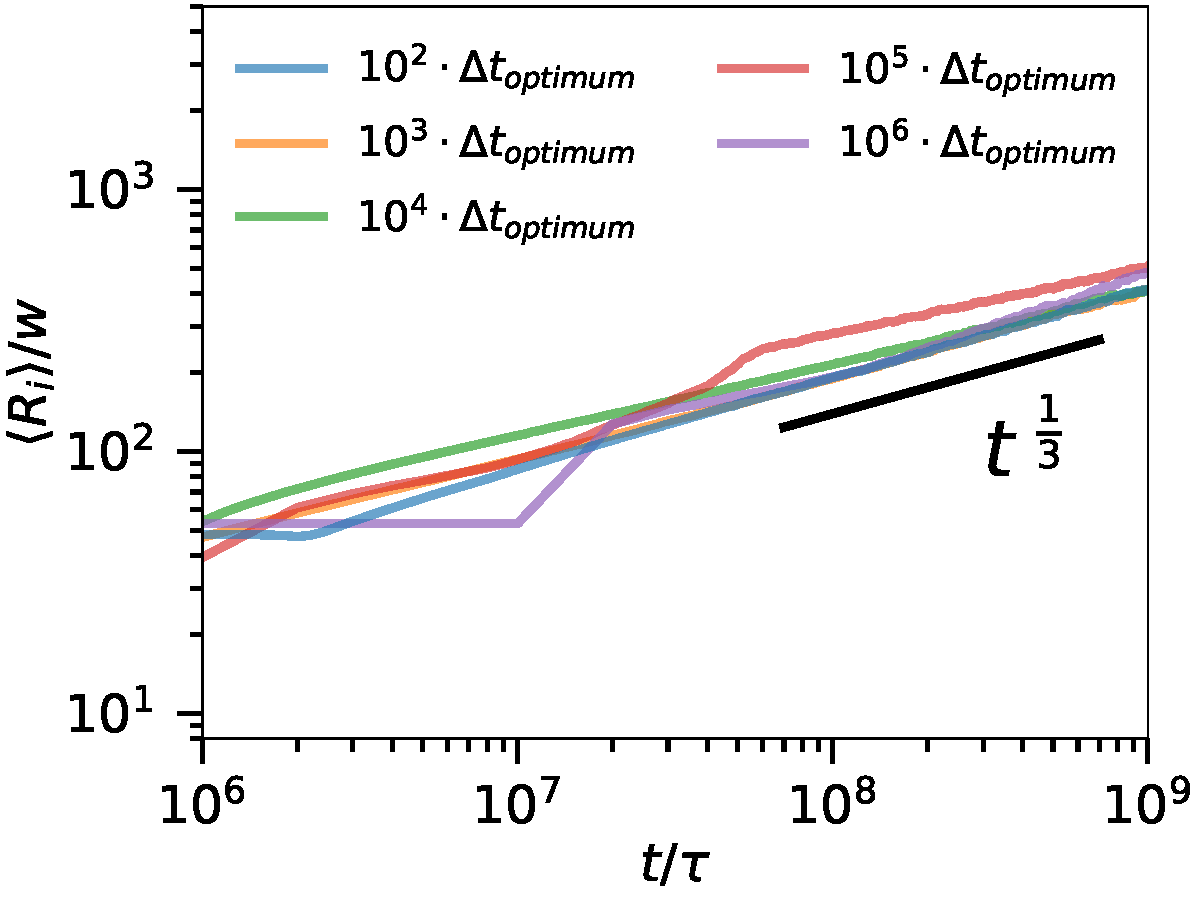
\includegraphics[scale=0.5]{MainContent/Figures/LSW_all.pdf}
\caption{\textbf{Effect of time-step $\dt$ on \textit{Ostwald-Ripening} in passive emulsions}.
Mean droplet radius $\langle R_i \rangle$ as a function of time $t$ shows the expected scaling $\langle R_i \rangle \propto t^{\,1/3}$; see Refs. \cite{Lifshitz,Wagner,LSWanalytics}, for low values of time-step $\dt$ and deviates strongly for higher $\dt$, thus validating our choice of the optimum time-step $\dt$ obtained from \Eqref{eqn:time_step}.
Remaining parameters are specified in Fig. \ref{fig:passive_emulsions}.
}
\label{fig:passive_emulsions_all}
\end{figure}

\section{Suppression of \textit{Ostwald-Ripening} in active emulsions}

As a final example for demonstrating the effective droplet model, we consider the interaction of many active droplets in a dilute emulsion.
In the case of simple first order reactions which convert droplet material $A$ into background field material $B$, \textit{Ostwald-Ripening} is suppressed and multiple droplets of a fixed size are produced; see Ref. \cite{Zwicker2015}.

% Such reactions are also present in biology, where $A,B$ can represent two states of a protein with their conversion facilitated by phosphorylation dephosphorylation reactions when the energy source is adenosine triphosphate molecules; see Ref. \cite{AlbertsBook2003}.
% Thus, simple reactions like these can be thought of as useful toy models and can provide insights into how the cell manages to regulate and finely tune the size of the condensates.

Generally speaking, in the case of first order reactions, we can argue towards the existence of a stable size for the droplets through balance between material fluxes inside and outside the droplet as follows:
droplet material is produced mainly in the background field and diffuses toward the droplet.
Inside the droplet, it gets destroyed due to chemical reactions which convert droplet material into background field material; which then diffuses into the background field.

As will be shown later, the total material flux inside the droplet $\vec{J}_\mathrm{in}$ scales as droplet volume, whereas the total material flux outside the droplet $\vec{J}_\mathrm{out}$ scales with the droplet radius.
Hence, we qualitatively expect the droplet to have a stable size based on the balances of the fluxes.
We elaborate on this point in the next section, where we study the effects of first order reactions on a single isolated droplet. 
Note that although the effective droplet model is formulated for generic reactions with complicated expressions for the reaction fluxes $s(\phiIn), s(\phiOut)$, here we focus on demonstrating the model for simple first-order reactions with linearized reaction fluxes which depend only on the composition.

We utilize a thin-interface description approach to formulate the dynamics of the volume fraction inside ($\phiIn$) and outside ($\phiOut$) the droplets; see Refs. \cite{Zwicker2015,Review2019}.
The chemical reaction scheme for the first-order reactions looks as:
\begin{equation}
\label{eqn:reaction_scheme}
    A \underset{\kf}{\stackrel{\kb}{\rightleftharpoons}} B,
\end{equation}
where droplet material A gets converted into background field material B inside the droplet with the rate $\kb$ and the background field material gets converted into droplet material inside the background field with the rate $\kf$.
Hence, the reaction flux in \Eqref{eqn:reaction_scheme} for both: inside the droplet and outside the droplet (i.e. inside the background field) reads as $s(\phi_\mathrm{in/out}) = \kf (1 - \phi_\mathrm{in/out}) - \kb \, \phi_\mathrm{in/out}$.
As we are interested in regimes where droplets are stable, we assume that local thermal equilibrium is quickly established and limit ourselves to regimes where $\kf, \kb$ are small as compared to the rate obtained from diffusion across the interface of the droplets given by $D_\mathrm{(in/out)} / w^2$; see Ref. \cite{Zwicker2015}.

First, we focus on the simple case of a single active droplet achieving a stable size, and then shift our attention to systems with multiple active droplets which exhibit suppression of \textit{Ostwald-Ripening}.

\subsection{Single active droplet in a large background field}
As mentioned before, active droplets can achieve a stable radius based on the balance of fluxes across the interface.
We aim to derive this stable radius for an active droplet with first-order chemical reactions immersed in a large background field, using the thin-interface approximation for the droplets; see Refs. \cite{Zwicker2015,Review2019}.

Similar to the case of a passive droplet in a large background field, we again assume strong phase separation and assume that $\phiIn,~\phiOut$ themselves vary little inside the droplet and the background field respectively.
Typically in a large system, chemical equilibrium is achieved far from the droplet when the reaction flux $s(\phi)=0$ and the average volume fraction is given by $\phi_\infty = \kf/(\kf + \kb)$; see Refs. \cite{Zwicker2015,Review2019}.

Consider an isolated active droplet of radius $R \gg w$ immersed in a large background field.
Owing to symmetry, we place a spherically symmetric co-ordinate system at the centre of the droplet with $r$ being the radial co-ordinate.
Since $\phiIn$ typically varies only a little, we use the thin-interface approximation; see \Eqsref{eqn:thin_interface_model}, of the continuous model to approximately arrive at the dynamical equation for $\phiIn$ as:

\begin{align} 
    \label{eqn:RD_droplet_firstorder}
    \frac{\partial \phiIn}{\partial t}
        \approx D_\mathrm{in} \nabla^2 \phiIn +
         \kf (1 - \phiIn) - \kb (\phiIn),
\end{align}
where $D_\mathrm{in}$ is the diffusivity inside the droplet.
We can analytically solve for $\phiIn$ from the stationary state of \Eqref{eqn:RD_droplet_firstorder}, using the boundary conditions $\phiIn(R) = \phiEqIn$ and $\partial_r \phiIn (0) = 0$ and obtain 
\begin{equation*}
    \phiIn(r) = \left (\phiEqIn - \phi_\infty \right ) \left( \frac{R}{r} \right ) \frac{\sinh \left(\frac{r}{\xi_\mathrm{in} }\right)}{\sinh \left(\frac{R}{\xi_\mathrm{in} }\right)} + \phi_\infty.
\end{equation*}

The solution reveals that $\phiIn$ increases monotonically inside the droplet till it attains a value $\phiEqIn$ and varies on the characteristic reaction-diffusion length-scale $\xi_\mathrm{in}=\sqrt{D_\mathrm{in}/({\kf + \kb})}$; see Ref. \cite{Review2019}.

Similar to inside the droplet, the volume fraction in the background field $\phiOut$ also typically varies a little and is hence described from the thin-interface approximation; see \Eqsref{eqn:thin_interface_model}, as:

\begin{align} 
    \label{eqn:RD_dilute_firstorder}
    \frac{\partial \phiOut}{\partial t}
        \approx D_\mathrm{out} \nabla^2 \phiOut +
         \kf (1 - \phiOut) - \kb \phiOut,
\end{align}
where $D_\mathrm{out}$ is the diffusivity outside the droplet.
Outside the droplet, we solve for $\phiOut$ from the stationary state of \Eqref{eqn:RD_dilute_firstorder}, using the boundary conditions $\phi_\mathrm{out}(R) = \phiEq_\mathrm{out}$ and $\phiOut(\infty) = \phi_\infty$.
We thus obtain 
\begin{equation*}
    \phiOut(r) =  [\phiEqOut - \phi_\infty] \left [ \frac{R}{r} \right ] e^{\left({\frac{R - r}{\xi_\mathrm{out}}}\right)} + \phi_\infty.
\end{equation*}
This solution also reveals that $\phiOut$ increases/decreases monotonically from $\phiEqOut$ to $\phi_\infty$ and varies on the characteristic reaction-diffusion length-scale, $\xi_\mathrm{out}=\sqrt{D_\mathrm{out}/({\kf + \kb})}$.
Simply put, $\phiOut$ reaches a value $\phi_\infty$ at a distance of roughly $\xi_\mathrm{out}$ from the droplet surface.
Thus, when we mean large systems, we consider system sizes $L$ which are $L \gg \xi_\mathrm{out}$, which is the definition we use in this thesis.
Consequently, finite systems would imply $L \sim \xi_\mathrm{out}$.

Spatial gradients in $\phiIn$ and $\phiOut$ at the droplet surface lead to local material fluxes outside the droplet as $\vec{j}_\mathrm{out} = [-D_\mathrm{out} {\boldsymbol{\nabla}} \phiOut (R)]$ and inside the droplet as $\vec{j}_\mathrm{in}  = [-D_\mathrm{in} {\boldsymbol{\nabla}} \phiIn (R)]$.
Note that, we typically assume same diffusivity $D$ inside and outside the droplets, i.e. $D_\mathrm{out} \approx D_\mathrm{in} = D$, which also implies $\xi_\mathrm{in} \approx \xi_\mathrm{out} = \xi$.
The fluxes then read as:
\begin{subequations}
\label{eqn:fluxes_in_firstorder}
\begin{align}
    \jIn \cdot \vec{n} &= D (\phiEqIn  - \phi_\infty) \left[ \frac{1}{R} - \frac{\coth \left (\frac{R}{\xi}\right )}{\xi} \right ] \mathrm{~and~}
    \\[10pt]
   \jOut \cdot \vec{n} &= 
    D (\phiEqOut  - \phi_\infty) \left[ \frac{1}{R} + \frac{1}{\xi} \right ].
\end{align}
\end{subequations}
We can now calculate the interfacial speed $v_n$ from \Eqref{eqn:InterfacialSpeed} and thus arrive at the stationary states for the droplet by numerically solving for $v_n = 0$.
This typically reveals two solutions $R_\ast, \overline{R}$ (as $\phiEqIn,~\phiEqOut$ depend on the droplet radius $R$; see \Eqsref{eqn:GibbsThompsonRelations}).

Droplets smaller than the critical radius $R_{\ast}$, defined as the radius at which the equilibrium volume fraction of the droplet equals the local supersaturation, dissolve quickly and is hence an unstable radius. 
On the other hand, droplets greater than $R > R_{\ast}$ grow until they reach the radius $\overline{R}$ and don't grow any further.
This follows from \Eqsref{eqn:fluxes_in_firstorder} as: For $R \ll \xi$, $\vec{J}_\mathrm{in} = \int_\Omega \jIn~\mathrm{d}A = 4 \pi R^2 \,\jIn$ scales with the volume of the droplet, which is seen from expanding the last term in $\jIn\cdot \vec{n}$ as $\left [\xi - R \coth \left (\frac{R}{\xi}\right ) \right ] \Big {/} (R \, \xi) \approx -R/(3\,\xi^2)$.
On the other hand, $\vec{J}_\mathrm{out} = \int_\Omega \jOut~\mathrm{d}A = 4 \pi R^2 \,\jOut$ scales with the radius of the droplet, which is seen from expanding the last term in $\jOut\cdot \vec{n}$.
Hence destruction of droplet material due to $\vec{J}_\mathrm{in}$ takes over if the droplet starts to grow bigger than $\overline{R}$.
The droplet then shrinks back to $\overline{R}$, thus indicating that this is the stable radius. 

Having numerically solved for the stable radius $\overline{R}$ after equating the fluxes from \Eqsref{eqn:fluxes_in_firstorder} for large systems, we now show that our effective droplet model agrees well with these predictions.
Indeed, as seen from Fig. \ref{fig:active_droplet_3D}A, the stable radius $\overline{R}_\mathrm{3D}$ (black line) obtained from the analytics ($\jIn = \jOut$ in \Eqsref{eqn:fluxes_in_firstorder}) compares well with simulations of the effective droplet model with optimum parameters (blue line) for large systems, but deviates from the continuous model (orange line).
This deviation occurs because $\overline{R}_\mathrm{3D}$ is a numerical solution from setting $\jIn = \jOut$ in \Eqsref{eqn:fluxes_in_firstorder}.
We simulate the effective droplet model for a single active droplet of initial radius $R_0 = 4w$ in a periodic 3 dimensional large system of size $[0, L_1]^3$, where $L_1 = 767w$.
We start with an initial background field $\phiOut(t=0) = \phi_\infty$, and the droplet grows until it reaches a stable radius.
Simulations using the continuous model were carried out for a droplet of initial radius $R_0 = 4w$ with $\phi(t=0) = \phi_\infty$ in a spherically symmetric domain of size $r \in [0, 5 \xi]$.
We choose optimum parameters, which in this case are $\dx \approx \ell \approx \ds \approx R_0$, as we desire to accurately model the vicinity of the droplet and the resulting fluxes.

\begin{figure}[tb]
\centering
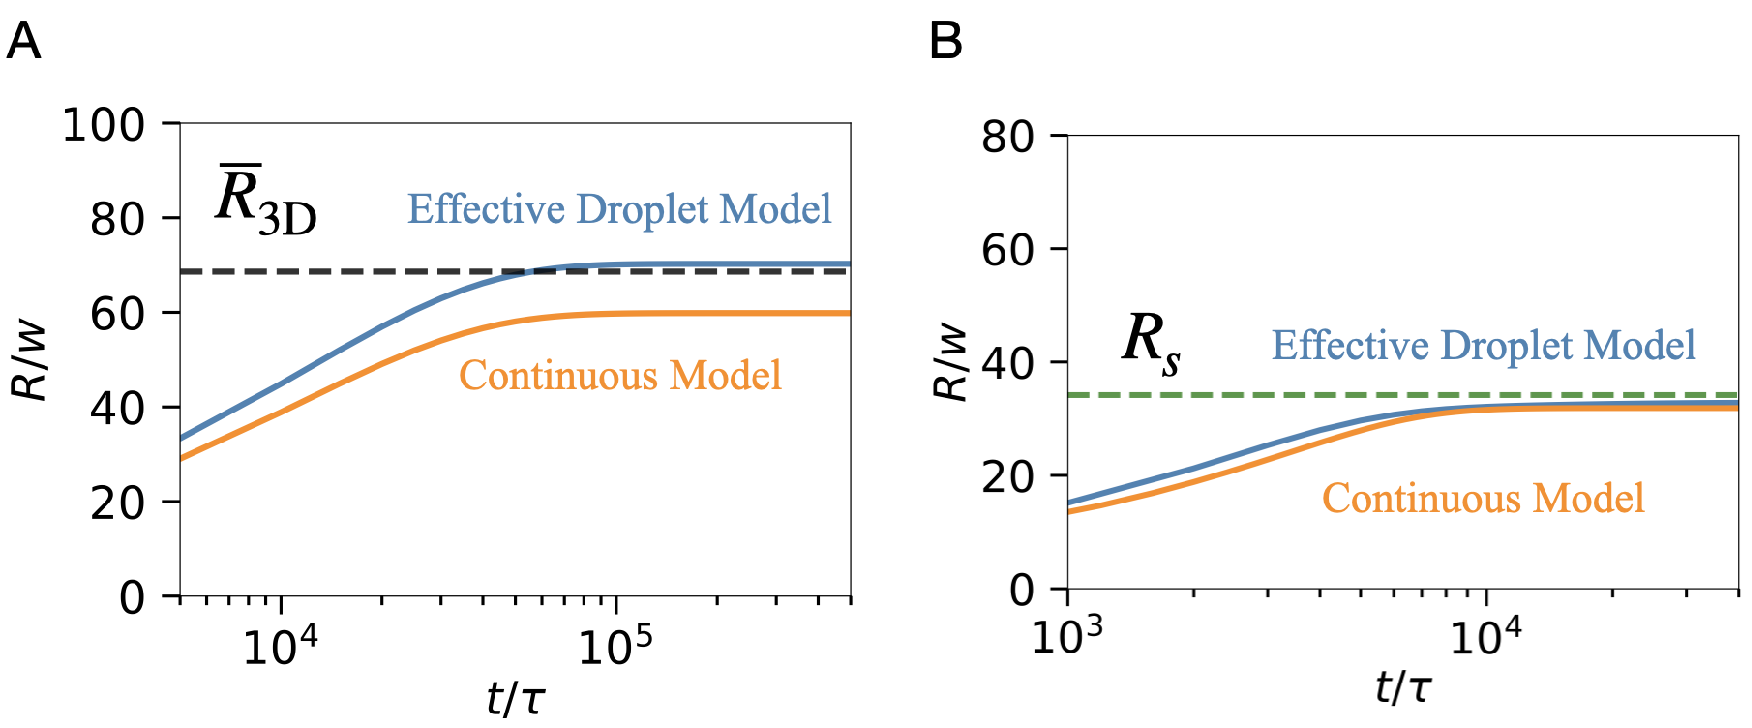
\includegraphics[scale=0.5]{MainContent/Figures/active_droplet_3D.pdf}
\caption{\textbf{Single active droplet reaches a stable radius in a large system (A) and a finite system (B).}
(A) Droplet radius $R$ as a function of time $t$.
The droplet reaches a fixed size $\overline{R}_\mathrm{3D}$ (dashed line) in a large system. 
$\overline{R}_\mathrm{3D}$ is obtained from numerically solving for $\jIn = \jOut$ from \Eqsref{eqn:fluxes_in_firstorder}, compares well with the effective droplet model (blue) and deviates from the continuous model (orange).
Simulations using the effective droplet model were carried out for a droplet of initial radius $R_0 = 4 w$ with $\phiOut(t=0) =\phi_\infty$ in a $3$-dimensional periodic cubic domain of size $[0, L_1]^3$, where $L_1 = 767w$ with $\dx \approx \ell \approx \ds \approx R_0$.
Simulations using the continuous model were carried out for a droplet of initial radius $R_0 = 4 w$ with $\phi(t=0) = \phi_\infty$ in a spherically symmetric domain of size $r \in [0, 5 \xi]$.
(B) Droplet reaches a fixed radius $R_s$ (dashed green line) given by \Eqref{eqn:approx_stable_radius_finite} for a finite system and compares well with simulations using the effective droplet model (blue) and using the continuous model (orange).
% Inset shows the volume fraction $\phi$ as a function of the radial co-ordinate $r$ from simulations of the continuous model at time $t = 4 \times 10^4 \tau$, with stable droplet radius $R_s$ (dashed green line) and $\phi = \phi_\infty$ (dashed black line).
% Far from the droplet, $\phi$ reaches a value which significantly lower than $\phi_\infty$, as is expected for a finite system.
Simulations using the continuous model were carried out for a droplet of initial radius $R_0 = 4 w$ with $\phi(t=0) =\phi_\infty$ in a spherically symmetric domain of size $r \in [0, 0.8 \xi]$.
Simulations using the effective droplet model were carried out with $\phiOut(t=0) = \phi_\infty$ in a $3$-dimensional periodic cubic domain of size $[0, L_2]^3$, where $L_2 = 122w$.
As $R_s$ is calculated from a mean-field approach, simulation parameters were $\dx \approx \ell \approx \ds \approx L_2$.
\mbox{(A-B)}
Model parameters are $s(\phi)= \kf (1 - \phi) - \kb \phi$, $\kf = 1 \times 10^{-5} \tau^{-1}$ and $\kb = 1 \times 10^{-4}  \tau^{-1}$.
Remaining parameters are specified in Fig. \ref{fig:droplet_pair_schematics}.
}
\label{fig:active_droplet_3D}
\end{figure}

We also simulate a single active droplet reaching it's fixed size for a large 2 dimensional system and compare it with the analytical predictions, too study how well the effective droplet model works for two dimensions.
As seen from Fig. \ref{fig:active_droplet_2D_infinite}, the stable radius $\overline{R}_\mathrm{2D}$ obtained from the analytical predictions ($\jIn = \jOut$ in \Eqsref{eqn:fluxes_in_firstorder}) compares well with simulations of the effective droplet model with optimum parameters.
We simulate the effective droplet model for a single active droplet of initial radius $R_0 = 4w$ in a periodic 2 dimensional large system of size $[0, L_1]^3$, where $L_1 = 843w$.
We start with an initial background field $\phiOut(t=0) = \phi_\infty$, and the droplet grows until it reaches a stable radius.
We choose optimum parameters as well, which in this case are $\dx \approx \ell \approx \ds \approx R_0$.
Simulations using the continuous model were carried out for a droplet of initial radius $R_0 = 4w$ with $\phi(t=0) = \phi_\infty$ in a polar domain of size $r \in [0, L_2]$, where $L_2 = 5 \xi$.

Additionally, it is again interesting to see that increasing approximations of the continuous model (in orange) lead to increasingly worse estimates for droplet drift, as the analytical predictions from the thin-interface approximation (dashed line); see \Eqsref{eqn:thin_interface_model}, are approximations of the continuous model, and the effective droplet model (in blue) is an approximation of \Eqsref{eqn:thin_interface_model}.

\begin{figure}[tb]
\centering
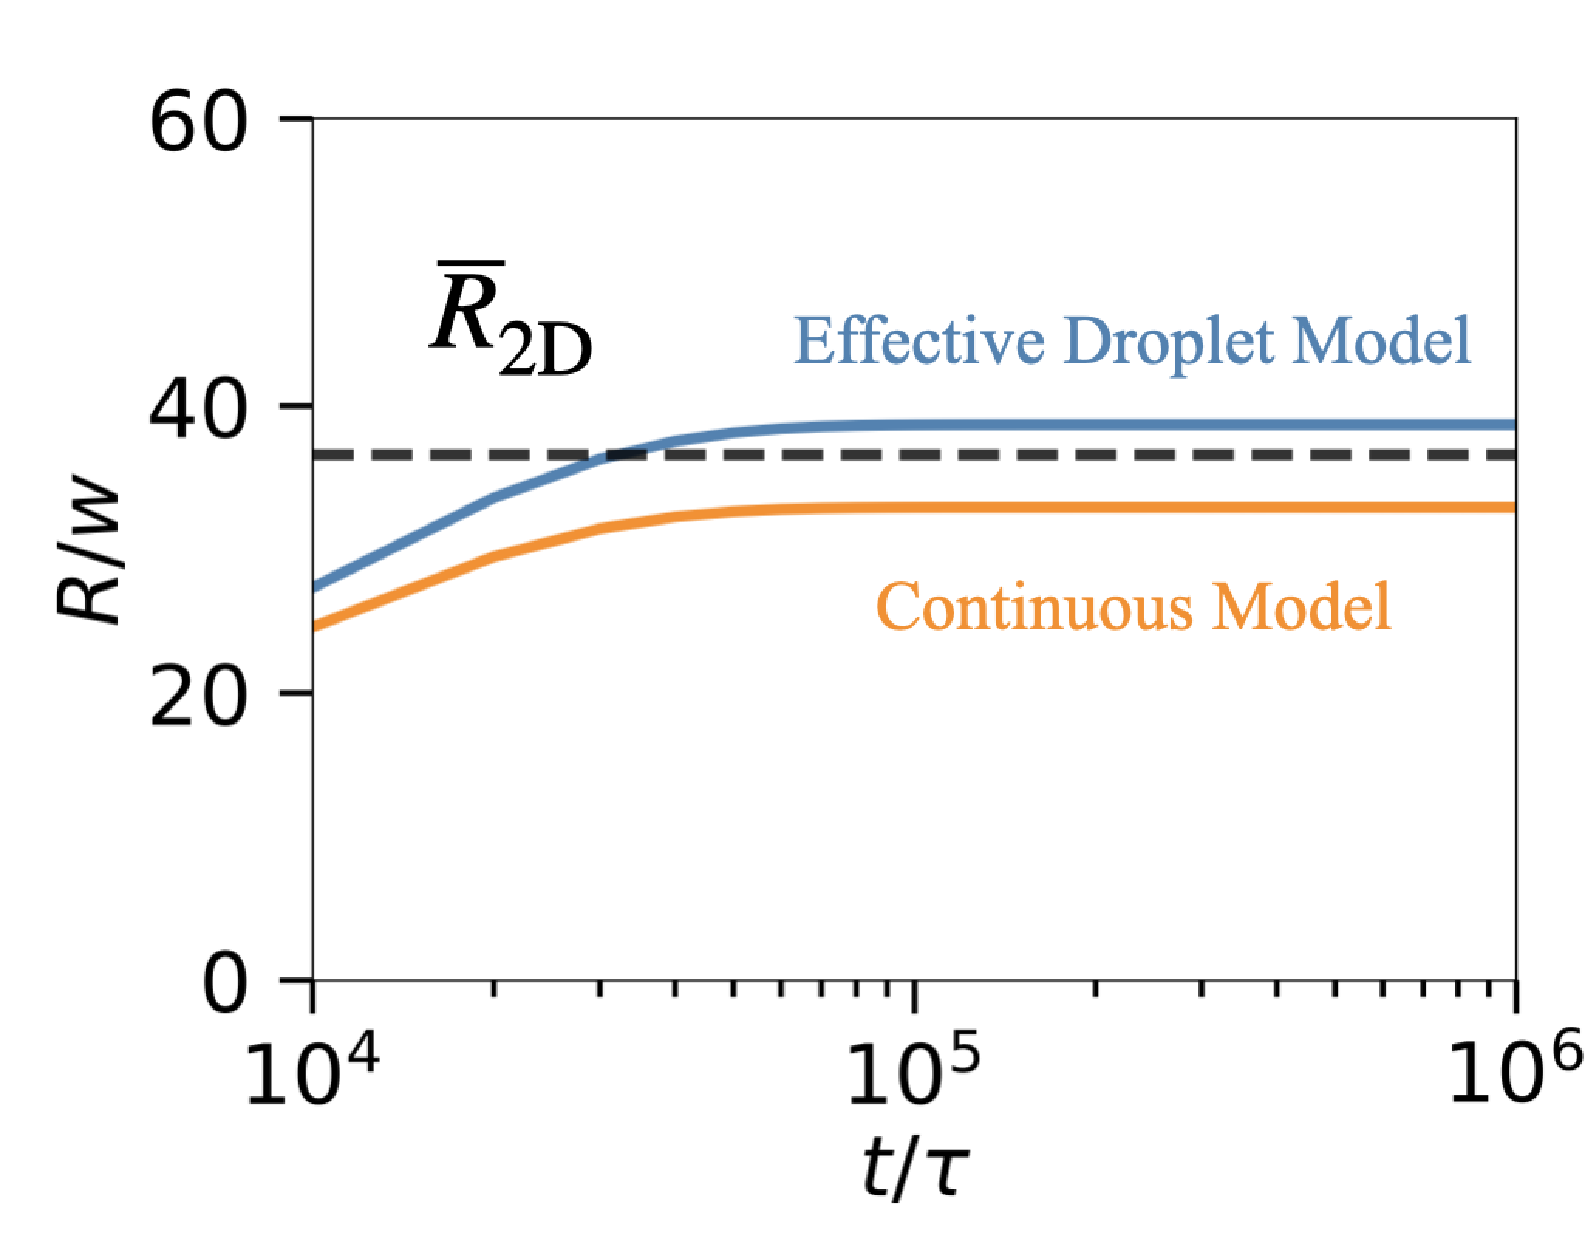
\includegraphics[scale=0.3]{MainContent/Figures/active_droplet_2D_infinite.pdf}
\caption{\textbf{Single active droplet reaches a stable radius in a large two dimensional systems.}
Droplet radius $R$ as a function of time $t$, which reaches a fixed size $R_\mathrm{2D}$ (dashed line) given by numerically solving for $\jIn = \jOut$ from \Eqsref{eqn:fluxes_in_firstorder} for 2 dimensions, and compares well with the effective droplet model (blue) and the continuous model (orange).
Simulations using the effective droplet model were carried out for a droplet of initial radius $R_0 = 4 w$ with $\phiOut(t=0) = \phi_\infty$ in a $2$-dimensional periodic square domain of size $[0, L_1]^2$, where $L_1 = 843 w$.
Simulation parameters were selected as $\dx \approx \ell \approx \ds \approx R_0$.
Simulations using the continuous model were carried out for a droplet of initial radius $R_0 = 4 w$ with $\phi(t=0) = \phi_\infty$ in a polar domain of size $r \in [0, L_2]$, where $L_2 = 5 \xi$.
Model parameters are $s(\phi)= \kf (1 - \phi) - \kb \phi$, $\kf = 1 \times 10^{-5} \tau^{-1}$ and $\kb = 1 \times 10^{-4}  \tau^{-1}$.
Remaining parameters are specified in Fig. \ref{fig:droplet_pair_schematics}.
}
\label{fig:active_droplet_2D_infinite}
\end{figure}

We next consider multiple interacting active droplets and their tendency to suppress \textit{Ostwald-Ripening}, eventually showing that simulations using the effective droplet model recover suppression of \textit{Ostwald-Ripening}.
Note that again we do not simulate this scenario using the continuous model, as it is computationally expensive. 
In this case too, we compare the effective droplet model with analytical predictions. 

\subsection{Multiple interacting active droplets and suppression of \textit{Ostwald-Ripening}}

Until now, we have shown that a single isolated active droplet reaches a stable radius $\overline{R}$ in a large system, which is calculated from a balance of the fluxes $\jIn,~ \jOut$ inside and outside the droplets from \Eqsref{eqn:fluxes_in_firstorder}.
However, a system of active droplets in a finite sized system can also reach a stable radius, effectively suppressing \textit{Ostwald-Ripening}, which amongst other parameters, depends on the reaction rates $\kf, \kb$, the system volume $V_\mathrm{system}$.

In this section, we briefly discuss the mean-field approach developed by Zwicker et al. \cite{Zwicker2015} and elaborate on the stable radius which multiple interacting active droplets in an emulsion attain.
Generally, in an emulsion of $N$ active droplets in a finite sized system, the supersaturation $\overline{\phi}$ in the system which is felt outside each droplet is $\overline{\phi} \leq \phi_\infty$.
This is in contrast to the case of a single active droplet because now the droplet material is limited and has to be shared amongst $N$ droplets.
We thus qualitatively expect the stable radius of the droplets in such a system to be lesser than $\overline{R}$.

The dynamics of $\overline{\phi}$ is governed by the simple reaction-diffusion equation, where we invoke the \textit{quasi-static approximation} and we assume that $\overline{\phi}$ relaxes quickly when compared with the droplet growth rates. 
Taking into account contributions from the droplets following \Eqref{eqn:reaction_scheme}, we arrive at the dynamical equation for $\overline{\phi}$ as:
\begin{equation}
\label{eqn:phi_dynamics}
    \partial_t \overline{\phi} = \kf (1- \overline{\phi}) - \kb (\overline{\phi}) + \frac{\sum_{i=1}^{N}~ \int_{\Omega_{i}} ~ \jIn\cdot \vec{n}}{V_\mathrm{system}},
\end{equation}
where the last term accounts for diffusive fluxes, $\Omega_i$ is the $i^\mathrm{th}$ droplet surface and $V_\mathrm{system}$ is the system volume, along with $V_\mathrm{system} \gg V_\mathrm{total}$. 

Thus, the dynamics of the droplets are still described by the fluxes obtained from  \Eqsref{eqn:fluxes_in_firstorder} and the droplet growth rate from \Eqref{eqn:InterfacialSpeed}, but now the volume fraction far from the droplets is governed by \Eqref{eqn:phi_dynamics}.
We thus arrive at a complete description for the dynamics of $N$ active droplets in a finite system of volume $V_\mathrm{system}$. 

Next, we turn our focus to calculating the fixed radius every droplet in such a system attains.
Consider a system of $N$ active droplets, all of which attain a common radius $R_s$.
The slowest rate of relaxation to such a state is given as:

\begin{equation}
\label{eqn:lambda}
    \lambda = \frac{D w}{6 R_s^3} - \frac{2 \kb}{3},
\end{equation}
which is obtained when a linear stability analysis is performed for \Eqref{eqn:phi_dynamics} and \Eqref{eqn:InterfacialSpeed} around $R_s$; see Refs. \cite{Zwicker2015,Review2019}.
Note that $\lambda$ does not contain any information about the number of droplets, as it considers only a mean-field coupling of the droplet and the background field. 
Furthermore, $\lambda < 0$ implies the steady state $R_s$ is stable, which means that all the droplets have to be greater than the threshold radius given as:
\begin{equation*}
    R_\mathrm{th} = \left [\frac{D w}{4 \kb} \right ] ^ {\frac{1}{3}},
\end{equation*}
obtained by setting $\lambda = 0$.
Thus, multiple droplets can have a stable size only if $R_s > R_\mathrm{th}$. 
In most cases, this condition is satisfied for sufficiently large $\kb$; see Ref. \cite{Zwicker2015}.

Hence, the value of $R_s$ all the $N$ droplets attain depends on the droplet density:
\begin{enumerate}
    \item If the droplet density is small, i.e. $N / V_\mathrm{system} \gg \xi ^ {-3}$, droplets do not significantly alter the volume fraction far from them $(\overline{\phi} \approx \phi_\infty)$; see \Eqref{eqn:phi_dynamics}, and thus the stable radius stays the same for a single active droplet in a large system, i.e. $R_s \approx \overline{R}$.
    Simply put, this means \textit{Ostwald-Ripening} is suppressed in such low density systems and each droplets attains a radius $R_s \approx \overline{R}$.

    \item If the droplet density is large, i.e. $N / V_\mathrm{system} \ll \xi ^ {-3}$, the stable radius $R_s$ is less than $\overline{R}$. 
    This is simply because the total amount of droplet material is limited, which is shared commonly between $N$ droplets.
    In principle, this supersaturation $\overline{\phi}$ is solved from the coupled equations \Eqref{eqn:phi_dynamics} and \Eqref{eqn:InterfacialSpeed}.
    However, we can approximately calculate $\overline{\phi}$ by arguing that the total volume of droplet material $V_\mathrm{system}~\phi_\infty$ is an upper bound for the total droplet volume, i.e. $N \, V_s \approx V_\mathrm{system} \, \phi_\infty$.
    The stable radius $R_s$ can then be simply calculated as:
    \begin{equation}
    \label{eqn:approx_stable_radius_finite}
        R_s = \left [\frac{3 V_s}{4 \pi}\right ]^{\frac{1}{3}},
    \end{equation}
    and thus \textit{Ostwald-Ripening} is again suppressed, but with droplets of a smaller size than $\overline{R}$.

\end{enumerate}
We can also qualitatively explain why does a system of $N$ active droplets with first-order reactions attain a state where all the droplets have the same radius given by $R_s$.
In the absence of chemical reactions, \textit{Ostwald-Ripening} is observed and droplets coarsen over time, which is also seen from \Eqref{eqn:lambda} - when chemical reactions are absent, $\lambda > 0$ and is proportional to the size of the droplets.
The primary reason for small droplets to shrink and big droplets to grow bigger is surface tension, as the material flux is directed from the smaller droplets (having a high value of $\phiEqOut$) towards the bigger droplets (having a low value of $\phiEqOut$).
However, in the case of first order reactions, surface tension effects will be countered by diffusive fluxes originating from the background field into the droplet due to chemical reactions and hence multiple droplets of the same size can co-exist.

Having developed a mean-field framework for calculating the fixed size for a system of $N$ active droplets, we aim to demonstrate that the effective droplet model is able to capture this fixed size which the droplets attain.
We choose three different mean-field coarsening scenarios in increasing complexity and compare simulations using the effective droplet model with the analytical predictions:

\begin{enumerate}
    \item A single active droplet in a finite system.
    
    \item A pair of active droplets coarsening in a large and a finite system.

    \item Multiple active droplets coarsening in a large and a finite system.
    \end{enumerate}

%%%%%%%%%%%%%%%%%%%%%%%%%%%%%%%%%%%%%%%%%%%%%%%%%%%%%%%%%%%%%%%%%%%%%%%%

\subsubsection{Coarsening of a single active droplet in a finite system}

We start by demonstrating that the effective droplet model captures the mean-field coarsening of a single active droplet in a finite system.
We simulate a droplet of initial radius $R_0 = 4 w$ embedded in an initial volume fraction $\phi_\infty = \kf/(\kf + \kb)$ and let it coarsen over time.
As seen from Fig. \ref{fig:active_droplet_3D}B, the droplet reaches a fixed radius $R_s$ (dashed green line) given by \Eqref{eqn:approx_stable_radius_finite} and compares well with simulations using the effective droplet model (blue) and using the continuous model (orange).
% Inset of Fig. \ref{fig:active_droplet_3D}B shows the volume fraction far from the droplet reaches $\phi \ll \phi_\infty$, as we correctly assumed.
Note that since the system size is small as compared to $\xi$, $\overline{R}_\mathrm{3D}$ (in black) is a poor estimate for the stable radius. 
Exploiting the symmetry of the problem, we use a spherically symmetric domain for the continuous model of size $r \in [0, 0.8 \xi]^3$ with $\phi(t=0) =\phi_\infty$.
Simulations using the effective droplet model were carried out with $\phiOut(t=0) = \phi_\infty$ in a $3$-dimensional periodic cubic domain of size $[0, L_2]^3$, where $L_2 = 122w$.
As $R_s$ is calculated from a mean-field approach, simulation parameters for the effective droplet model were chosen as $\dx \approx \ell \approx \ds \approx L_2$.

Additionally, it is again interesting to see that increasing approximations of the continuous model (in orange) lead to increasingly worse estimates for droplet drift, as the analytical predictions from the thin-interface approximation (dashed line); see \Eqsref{eqn:thin_interface_model}, are approximations of the continuous model, and the effective droplet model (in blue) is an approximation of \Eqsref{eqn:thin_interface_model}.

%%%%%%%%%%%%%%%%%%%%%%%%%%%%%%%%%%%%%%%%%%%%%%%%%%%%%%%%%%%%%%%%%%%%%%%%

\subsubsection{Coarsening of a pair of active droplets coarsening in a large system and a finite system}

Next, we demonstrate that the effective droplet model captures the mean-field coarsening of a pair of active droplets in: a) Large system and b) Finite system. 
We simulate two droplets of initial radius $R_0 = [20w, 80w]$ immersed again in a supersaturation equal to $\phi_\infty$, and let them coarsen over time.
Simulations using the effective droplet model were carried out for a pair of droplets, of initial radius $R_0 = [20w, 80w]$ in a $3$-dimensional periodic cubic domain of size $[0, L_1]^3$ for a finite system, where $L_1 = 200 w$ and size $[0, L_2]^3$ for a large system, where $L_2 = 10^4 w$.
As $R_s$ is calculated from a mean-field approach, simulation parameters were $\dx \approx \ell \approx \ds \approx L_1$ for the finite system and  $\dx \approx \ell \approx \ds \approx L_2$ for a large system.
Note that we do not simulate this system with the continuous model, owing to computational costs.

Fig. \ref{fig:active_droplet_pair}A shows that the droplets in the finite system reach a fixed radius $R_s$ (dashed green line) given by \Eqref{eqn:approx_stable_radius_finite} and compares well with simulations using the effective droplet model (blue).
The deviation of the stable radii from $\overline{R}_\mathrm{3D}$ is strong and expected, as $\overline{R}_\mathrm{3D}$ is analytically calculated for large systems.
On the contrary, Fig. \ref{fig:active_droplet_pair}B shows a good agreement of the effective droplet model with the theoretically predicted $\overline{R}_\mathrm{3D}$ for the droplet pair in a large system.

\begin{figure}[tb]
\centering
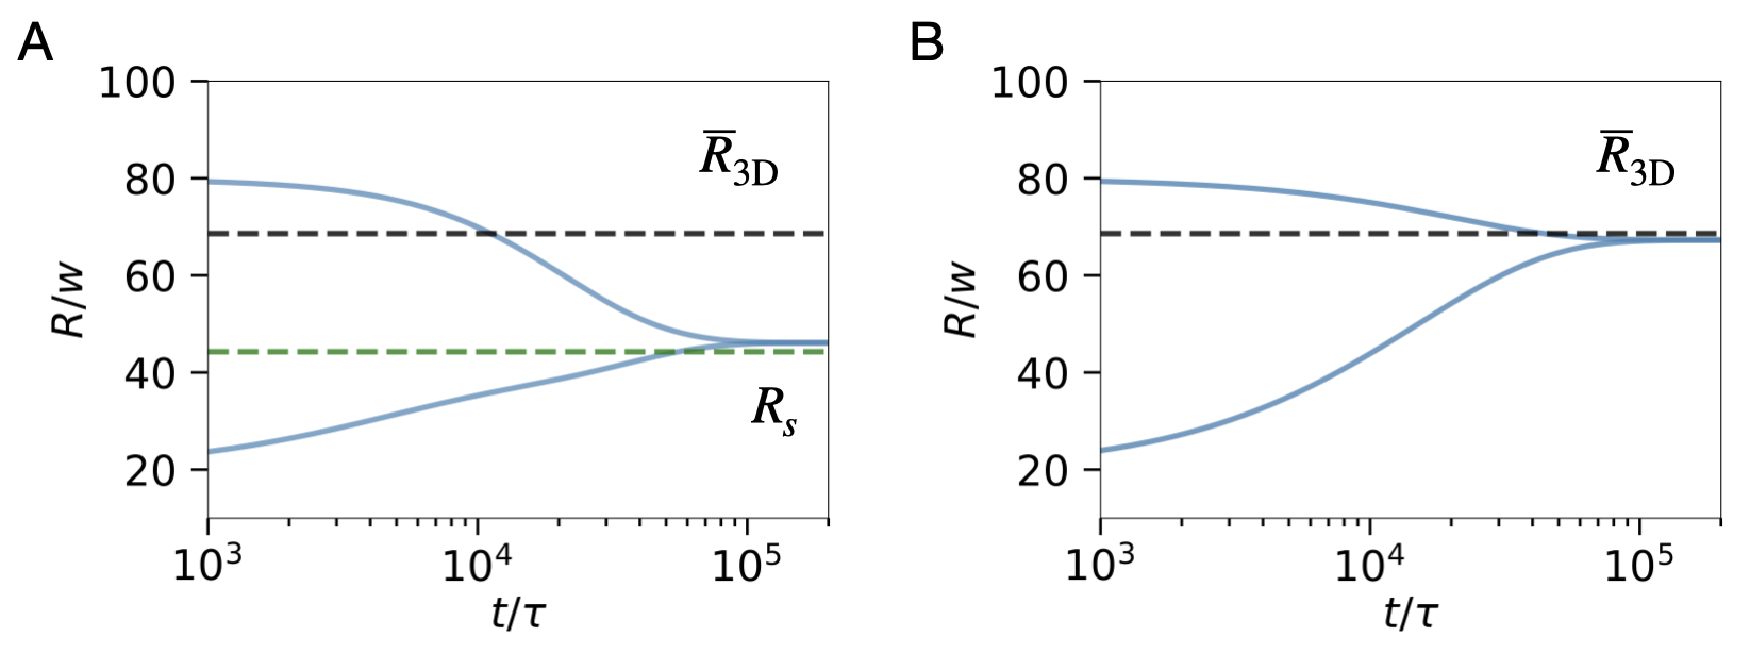
\includegraphics[scale=0.5]{MainContent/Figures/active_droplet_pair.pdf}
\caption{\textbf{Mean-field coarsening of a pair of active droplets in a finite system (A) and a large system (B).}
(A) Droplet radius $R$ as a function of time $t$ for a pair of active droplets in a finite system, which reaches a fixed size $R_s$ (dashed green line) predicted from \Eqref{eqn:approx_stable_radius_finite}, and compares well with the effective droplet model (blue).
(B) The droplet pair reaches a fixed radius $\overline{R}_\mathrm{3D}$ (dashed black line) given by numerically solving for $\jIn = \jOut$ from \Eqsref{eqn:fluxes_in_firstorder} for a large system and compares well with simulations using the effective droplet model (blue).
\mbox{(A-B)}
Simulations using the effective droplet model were carried out for a pair of droplets, of initial radius $R_0 = [20w, 80w]$ in a $3$-dimensional periodic cubic domain of size $[0, L_1]^3$ for a finite system, where $L_1 = 200 w$ and size $[0, L_2]^3$ for a large system, where $L_2 = 10^4 w$.
Model parameters are $s(\phi)= \kf (1 - \phi) - \kb \phi$, $\kf = 1 \times 10^{-5} \tau^{-1}$, $\kb = 1 \times 10^{-4}  \tau^{-1}$ and $\phiOut(t=0) = \phi_\infty$.
As $R_s$ is calculated from a mean-field approach, simulation parameters were $\dx \approx \ell \approx \ds \approx L_1$ for (A) and  $\dx \approx \ell \approx \ds \approx L_2$ for (B).
Remaining parameters are specified in Fig. \ref{fig:droplet_pair_schematics}.
}
\label{fig:active_droplet_pair}
\end{figure}
Thus our model successfully demonstrates the coarsening of a pair of droplets and agrees well with the analytical predictions and the continuous model.
Next, we consider slightly complex situations of multiple active droplets.

%%%%%%%%%%%%%%%%%%%%%%%%%%%%%%%%%%%%%%%%%%%%%%%%%%%%%%%%%%%%%%%%%%%%%%%%

\subsubsection{Coarsening of multiple active droplets in a large system}

We consider the interaction of many active droplets in a large dilute system and simulate $100$ droplets with radii uniformly chosen in $[10w, 50w]$ and placed in a periodic cubic domain of size $[0, L]^d$ with $L=1000 w$ in an initial supersaturation equal to $\phi_\infty$.

\figref{fig:active_emulsions}, \figref{fig:active_emulsion_1D} show that the emulsions with broad initial sizes quickly converge to a mono-disperse  distributions for $1, 2$ and $3$ dimensional systems.
The stable radii $\overline{R}_\mathrm{1D}, \overline{R}_\mathrm{2D}, \overline{R}_\mathrm{3D}$ are obtained from setting $\jIn = \jOut$ in \Eqsref{eqn:fluxes_in_firstorder} and they compare well with simulations using the effective droplet model.
Note that we do not use the continuous model for comparison, as it is extremely computationally costly, given the sizes of the system which we simulate. 

\begin{figure}[tb]
\centering
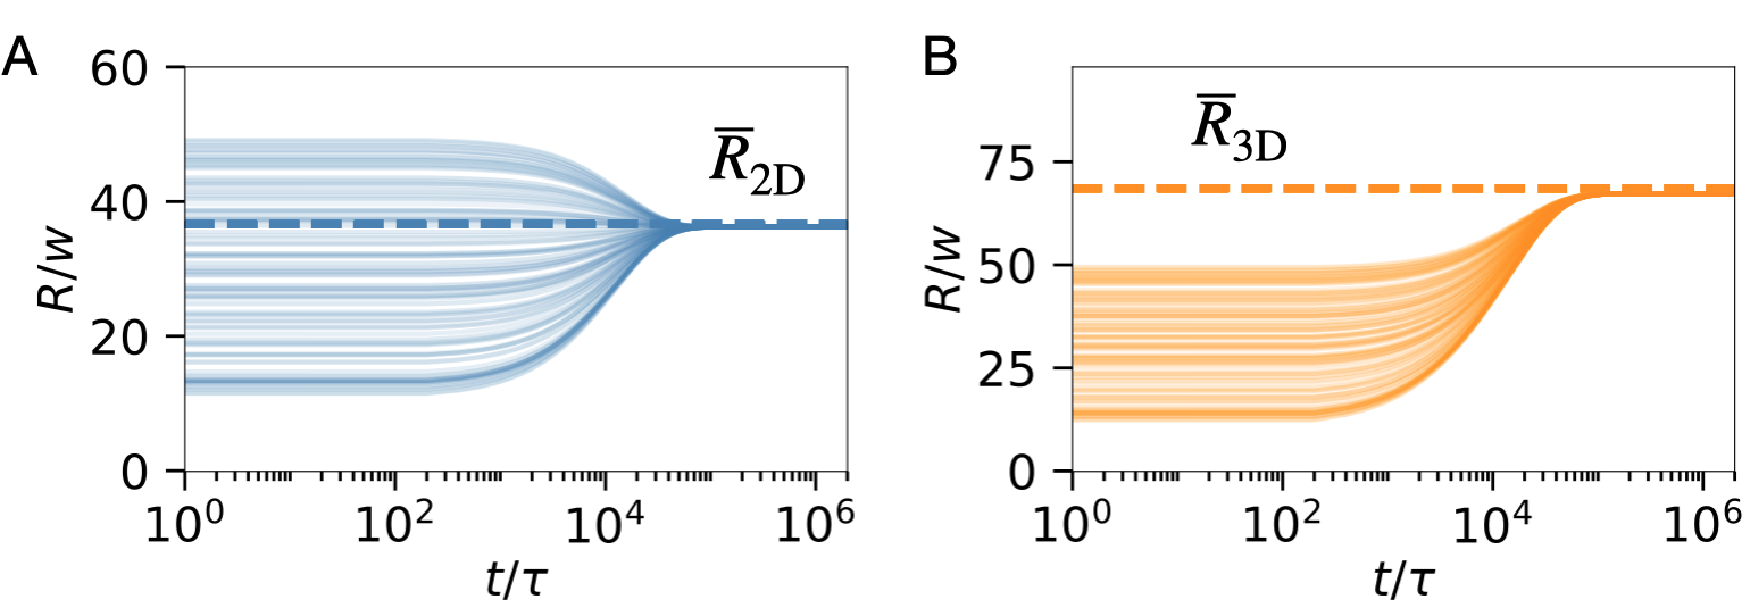
\includegraphics[scale=0.5]{MainContent/Figures/active_emulsions.pdf}
\caption{
\textbf{Suppression of \textit{Ostwald-Ripening} by first-order chemical reactions}.
%Active droplets with first-order chemical reactions attain a stationary radius based on material flux balance between incoming fluxes into the droplets and material destroyed inside the droplets.
(A, B) Radii $R$ as a function of time $t$ of droplets evolving in $d=2$ dimensions (A) and $d=3$ dimensions (B).
The theoretically expected radii are indicated by dashed horizontal lines for 2 dimensions as ($\overline{R}_\mathrm{2D}$) and for 3 dimensions as ($\overline{R}_\mathrm{3D}$). 
$\overline{R}_\mathrm{2D}, \overline{R}_\mathrm{3D}$ are obtained by numerically solving for $\jIn = \jOut$ from \Eqsref{eqn:fluxes_in_firstorder}.
$100$ droplets with radii chosen uniformly in $[10w, 50w]$ were placed in a periodic cubic domain of size $[0, L]^d$ with $L=1000 w$.
Model parameters are $s(\phi)= \kf (1 - \phi) - \kb \phi$, $\phiOut(t=0) =\phi_\infty$, $\kf = 1 \times 10^{-5} \tau^{-1}$, $\kb = 1 \times 10^{-4}  \tau^{-1}$, $\Delta x \approx \ell \approx L$, and a single shell sector for all droplets.
Remaining parameters are specified in Fig. \ref{fig:droplet_pair_schematics}.
}
\label{fig:active_emulsions}
\end{figure}

\begin{figure}[tb]
\centering
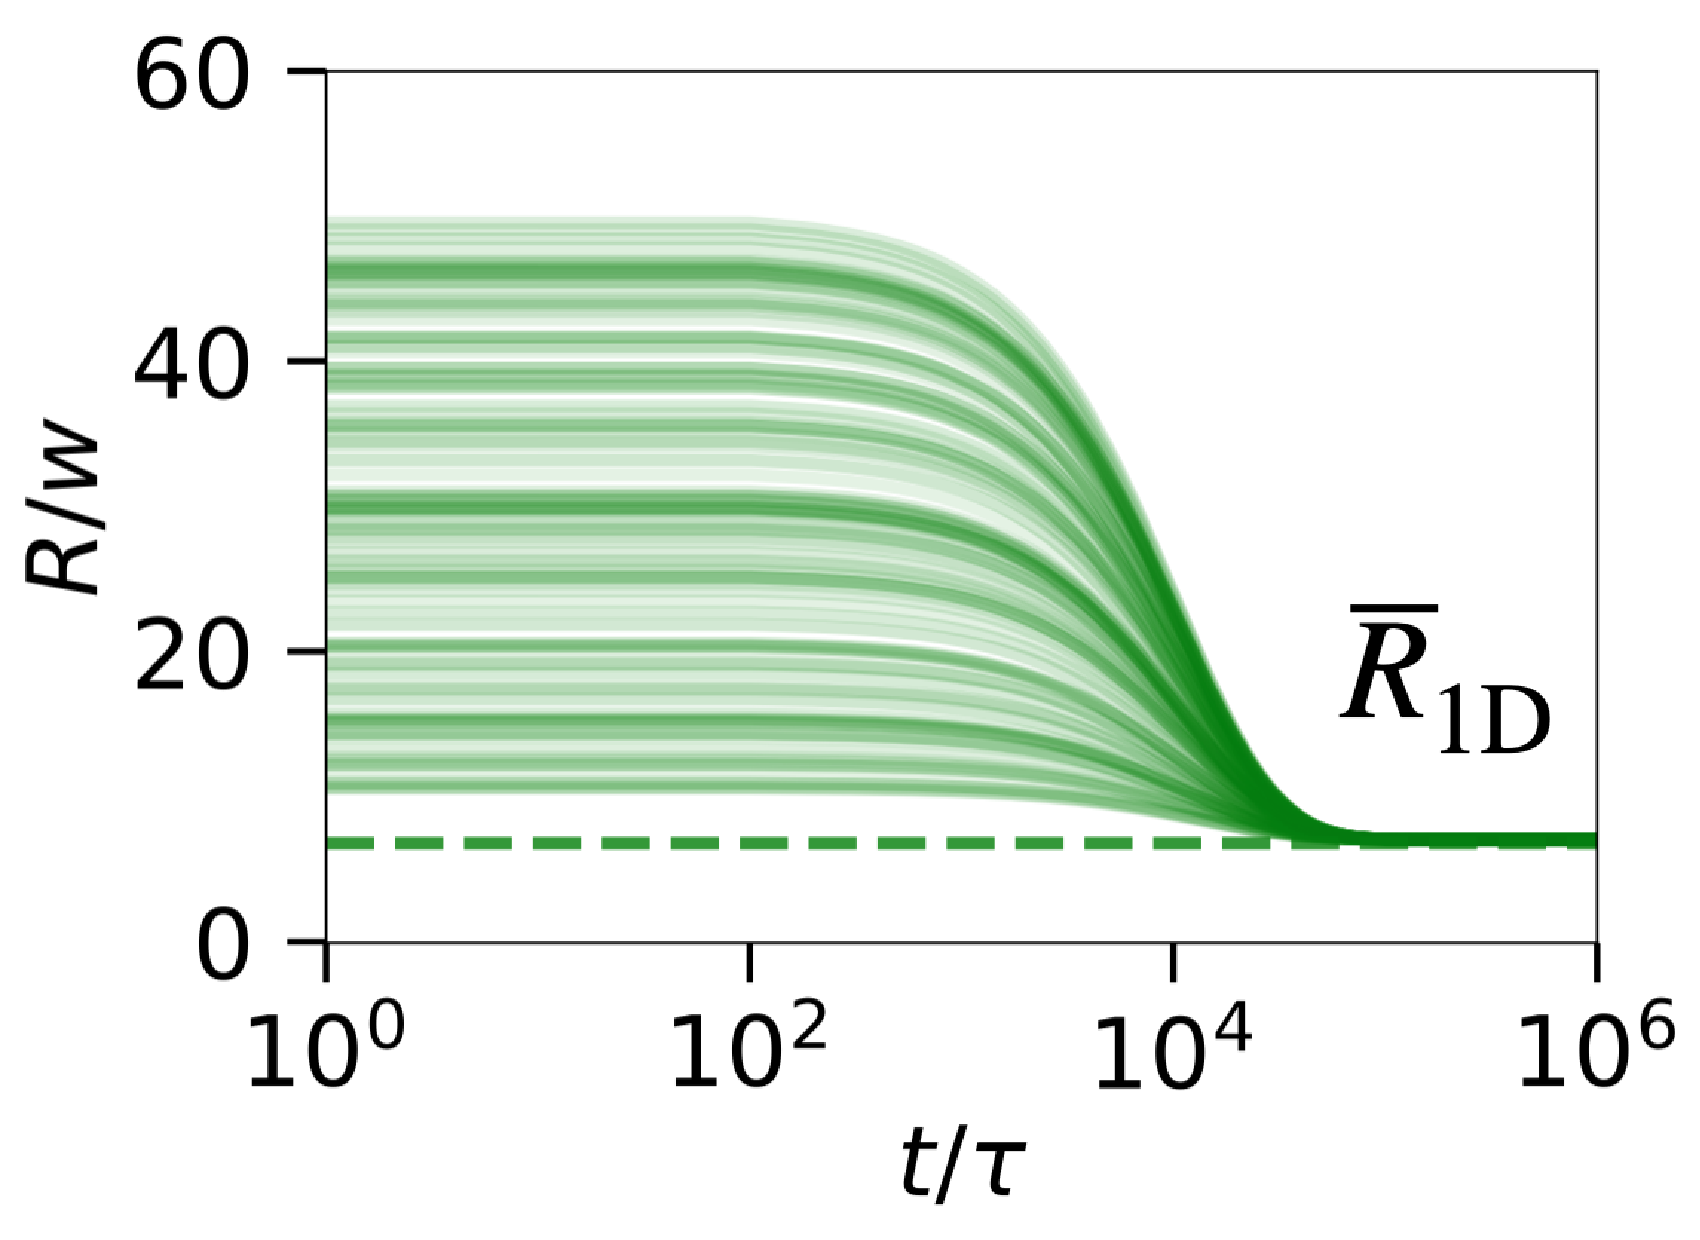
\includegraphics[scale=0.24]{MainContent/Figures/active_emulsion_1D.pdf}
\caption{
\textbf{Suppression of \textit{Ostwald-Ripening} by first-order chemical reactions in one dimension}.
Droplet radii $R$ as a function of time $t$ of active droplets evolving in $d=1$ dimension.
The theoretically expected radius is indicated by dashed horizontal line.
$100$ droplets with radii chosen uniformly in $[10w, 50w]$ are placed in a periodic one-dimensional Cartesian domain of size $[0, L]$ with $L=1000 w$.
Remaining parameters are specified in Fig. \ref{fig:active_emulsions}.
}
\label{fig:active_emulsion_1D}
\end{figure}

%%%%%%%%%%%%%%%%%%%%%%%%%%%%%%%%%%%%%%%%%%%%%%%%%%%%%%%%%%%%%%%%%%%%%%%%

\subsubsection{Coarsening of multiple active droplets in a finite system}

As a final example, we consider the interaction of many active droplets in a finite system.
It is known that multiple interacting active droplets undergoing first-order reactions typically arrange themselves in a hexagonal lattice for 2 dimensional systems; see Ref. \cite{Zwicker2015}, and as shown from simulations of the continuous model; see \figref{fig:lattice_2D_CH}.
In the steady state the droplets position themselves such that all of them share a common supersaturation $\overline{\phi}$ given by \Eqref{eqn:phi_dynamics}.
We now seek to recapitulate this phenomena using the effective droplet model.
Note that we do not simulate such systems using the continuous model, owing to prohibitive computational costs.

We simulate the effective droplet model for 10 droplets (\figref{fig:lattice_2D}A) and 40 droplets (\figref{fig:lattice_2D}C) of initial radius $R_0$ chosen uniformly in $[9.5w, 10.5w]$ in a periodic 3 dimensional system of size $[0, L]^2$, where $L = 10^3 w$.
We start with an initial background field $\phiOut(t=0) = \phi_\infty$, and the droplets grow until a stable radius is reached.
As we are primarily interested in the spatial resolution on a droplet level, we resolve $\phiOut$ on the scale of a single droplet.
This also ensures that the drift of the droplets is also captured correctly, which is an important factor in the formation of the lattice.

\begin{figure}[tb]
\centering
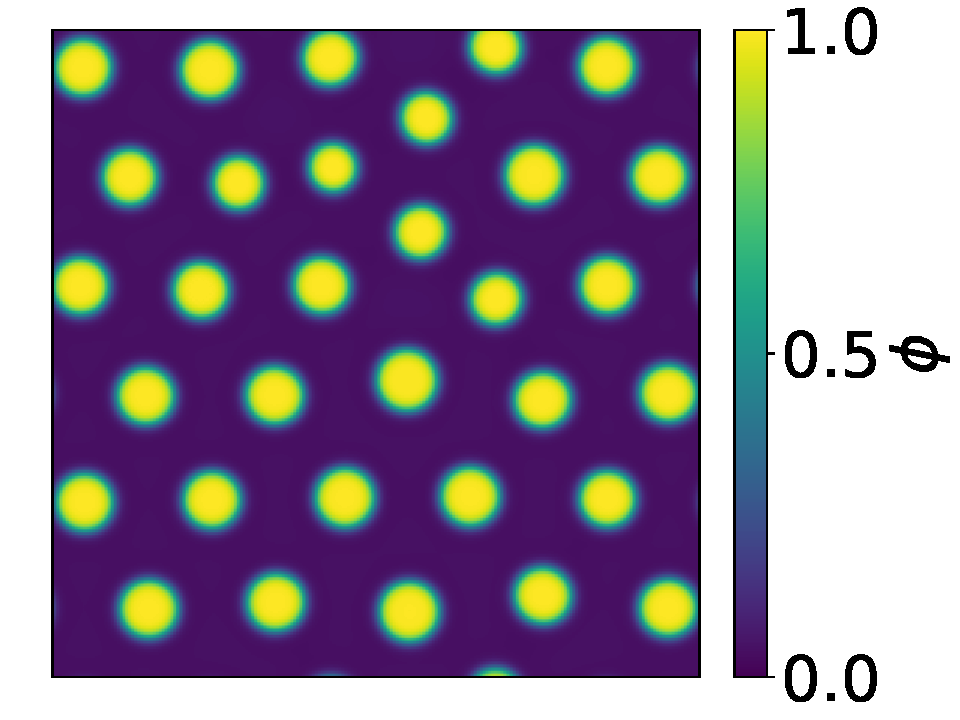
\includegraphics[scale=0.4]{MainContent/Figures/lattice_2D_CH.pdf}
\caption{\textbf{Active droplets with first order reactions forming a 2 dimensional lattice using the continuous model.}
Simulations using the continuous model shows active droplets forming a lattice in a 2 dimensional system using first-order reactions; see Ref. \cite{Zwicker2015}.
The continuous model used a $2$-dimensional periodic Cartesian domain of size $[0, L]^2$, where $L = 10^3 w$.
Model parameters are $s(\phi)= \kf (1 - \phi) - \kb \phi$, $\phi(t=0)$ is chosen as a random uniform field $\phi \in [0.1, 0.4]$ on the entire domain, $\kf = 3 \times 10^{-4} \tau^{-1}$, $\kb = 1 \times 10^{-3}  \tau^{-1}$.
Remaining parameters are specified in Fig. \ref{fig:droplet_pair_schematics}.
}
\label{fig:lattice_2D_CH}
\end{figure}

As seen from \figref{fig:lattice_2D}A and \figref{fig:lattice_2D}C, we recover this phenomena for a 2 dimensional finite system with different initial conditions consisting of increasing droplet number.
Furthermore, the stable radius $R_s$ predicted from \Eqref{eqn:approx_stable_radius_finite} agrees well with the effective droplet model, as seen from \figref{fig:lattice_2D}B and \figref{fig:lattice_2D}D, and deviates increasingly from $\overline{R}_\mathrm{2D}$ given by numerically solving for $\jIn = \jOut$ from \Eqsref{eqn:fluxes_in_firstorder}, with increasing droplet density.
This is expected, as the prediction for $\overline{R}_\mathrm{2D}$ assumes droplet density to be low.
For the simulations with low droplet density (\figref{fig:lattice_2D}A, \figref{fig:lattice_2D}B), $R_s > \overline{R}_\mathrm{2D}$ as $V_s = \pi R^2_s$ (for two dimensions) is directly proportional to the system volume $V_\mathrm{system}$ and hence will approach a large number as the system size $L \rightarrow \infty$.
Consequently, for simulations with high droplet density (\figref{fig:lattice_2D}C, \figref{fig:lattice_2D}D), $R_s < \overline{R}_\mathrm{2D}$ as $\overline{R}_\mathrm{2D}$ assumes the system size to be large. 
This interesting interplay between $R_s, \overline{R}_\mathrm{2D}$ is also seen from \figref{fig:lattice_2D}B, \figref{fig:lattice_2D}D.
Taken together, we in this section, we demonstrated that our effective model faithfully recovers important physical behaviour of active droplets.

\begin{figure}[tb]
\centering
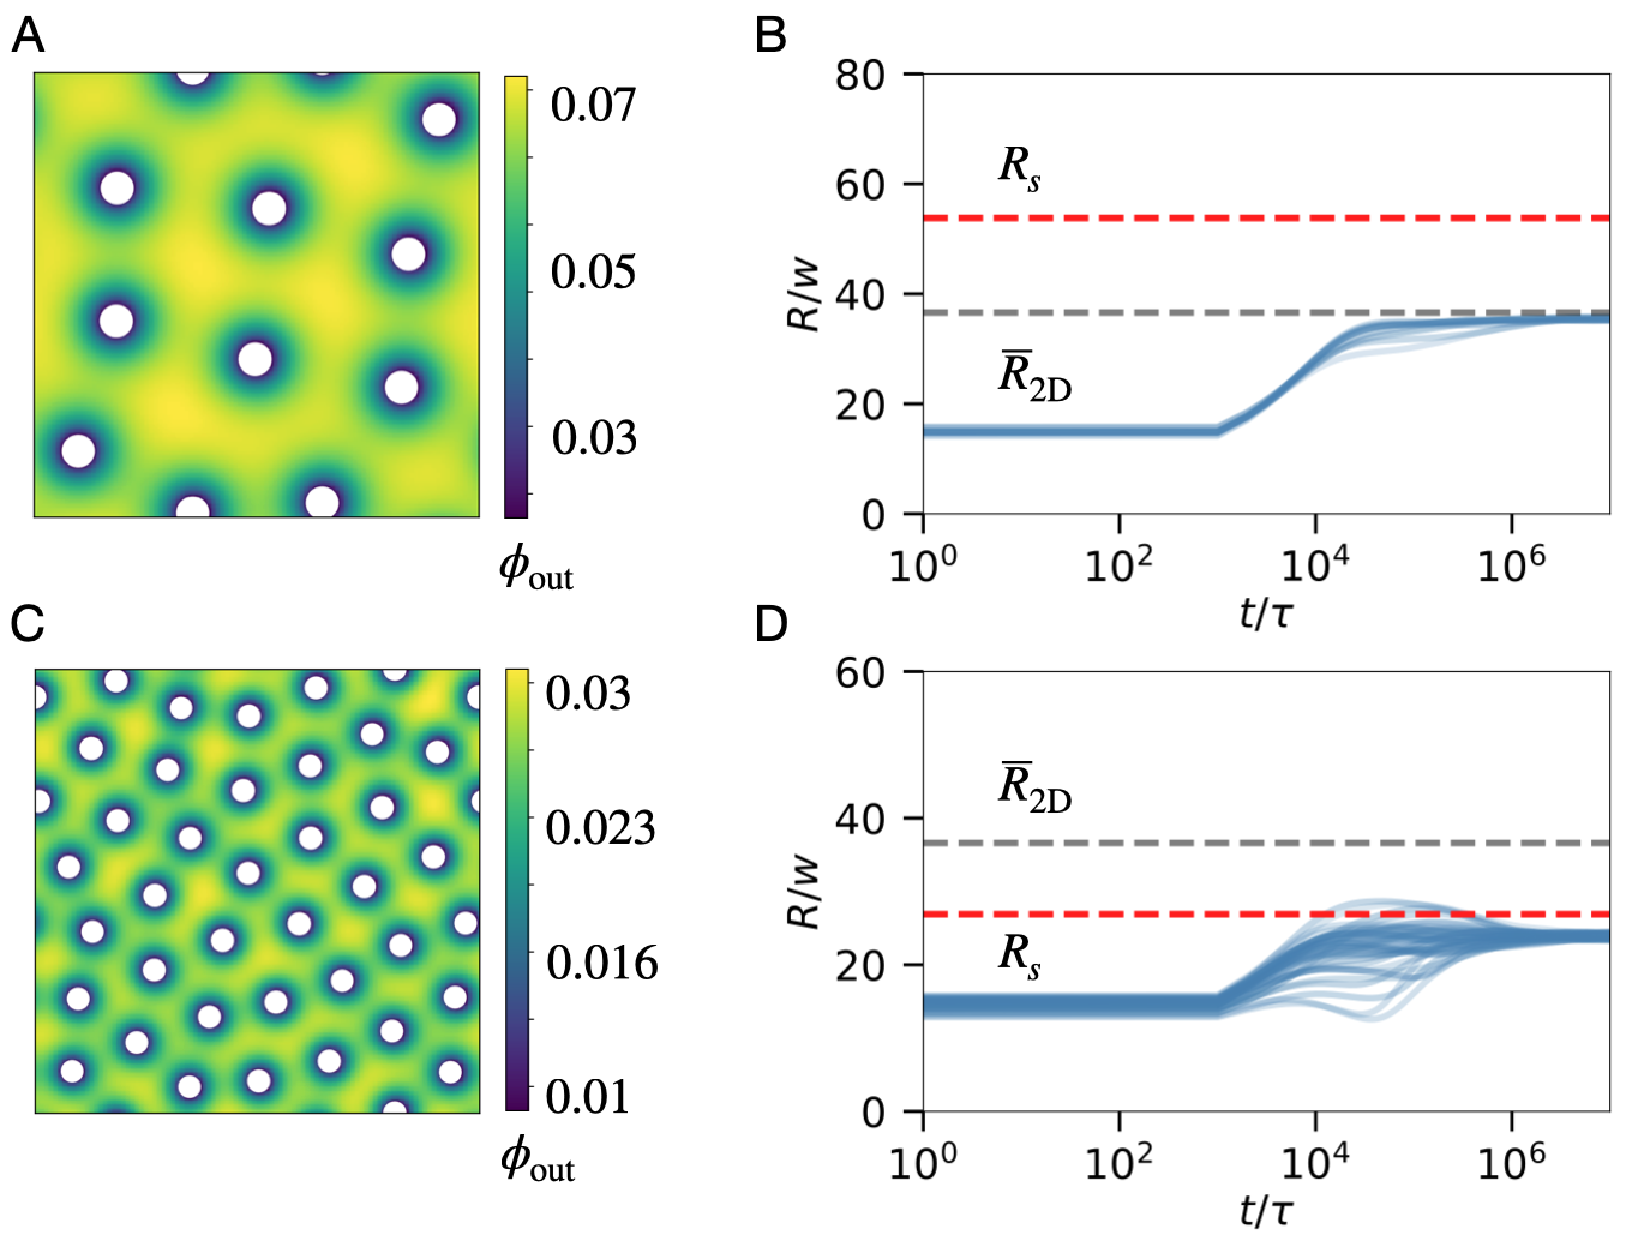
\includegraphics[scale=0.5]{MainContent/Figures/lattice_2D.pdf}
\caption{\textbf{Active droplets with first order reactions forming a two dimensional lattice using the effective droplet model.}
Active droplets with first-order chemical reactions attain a stationary radius and form a lattice in 2 dimensional systems using the effective droplet model.
(A) and (C) show 10 and 40 active droplets with radii chosen uniformly in $[9.5w, 10.5w]$ and placed in a periodic Cartesian domain of size $[0, L]^2$ with $L=10^3 w$.
(B) and (D) show droplet radius $R$ with time and a good agreement of the stable radius from the effective droplet model with the theoretically predicted $R_s$ (dashed red line) from \Eqref{eqn:approx_stable_radius_finite}. 
$\overline{R}_\mathrm{2D}$ (dashed black line), given by numerically solving for $\jIn = \jOut$ from \Eqsref{eqn:fluxes_in_firstorder}, deviates increasingly from $R_s$, for increasing droplet densities.
Model parameters are $s(\phi)= \kf (1 - \phi) - \kb \phi$, $\phiOut(t=0) =\phi_\infty$, $\kf = 1 \times 10^{-5} \tau^{-1}$, $\kb = 1 \times 10^{-4}  \tau^{-1}$, $\Delta x \approx \ds \approx \ell \approx R_0$.
Remaining parameters are specified in Fig. \ref{fig:droplet_pair_schematics}.
}
\label{fig:lattice_2D}
\end{figure}

\section{Summary}

In the last chapter; Chapter \ref{chap:Chapter_4}, we formulated the effective droplet model in detail which governs droplet dynamics according to \Eqsref{eqn:DropletDiscretized} and the dynamics of the background field $\phiOut$ using \Eqref{eqn:RD_dilute}.
We then put forward the numerical algorithm; see Algorithm \ref{alg:algorithm}, and used a test-case of a pair of identical passive droplets shrinking in a vanishing volume fraction to conclude that the optimum values for the effective droplet model are $[\dx \approx \ell \approx \ds]$.

In this chapter, we validated our claim of optimum simulation parameters for the effective droplet model by comparing it with known analytical results from literature and simulations using the continuous model (wherever computationally viable).
We were motivated from biology, in particular, simulating two mechanisms the cell potentially uses to regulate the dynamics of condensates - chemical reactions and external chemical gradients.
To help disentangle the individual roles of these two mechanisms, we considered them separately; first in simulations of single droplet systems, and then through simulations of many droplet systems. 

We started by considering simple scenarios involving a single droplet and moved to more complex situations, eventually reaching a point where we simulated coarsening behaviour of $10^5$ droplets.
As our aim was to simulate dynamics of phase separated droplets accurately, throughout all the simulation scenarios, we primarily focused on comparing droplet growth and drift.
Wherever possible, we derived the equations for growth (and drift) of the droplets using the thin-interface approximation given by \Eqsref{eqn:thin_interface_model}.

First, we simulated a passive droplet growing in a large supersaturated system and simulations using the continuous model, the effective droplet model with optimum parameters and analytical predictions; see Refs. \cite{Review2019,Weber2017}, match well; see \figref{fig:passive_droplet}.
Next, we validated the effective droplet model for a passive droplet in an external volume fraction gradient; see \figref{fig:drop_in_gradient} and tested the effective droplet model for this scenario for simulation parameters other than the optimum values, thus highlighting the importance of choosing the correct values for the simulation parameters; see \figref{fig:drop_in_gradient_all}.

We then moved on to demonstrate the hallmark of this model - the ability to simulate large scale emulsions of many droplets. 
To this end, we simulated \textit{Ostwald-Ripening}; see \figref{fig:passive_emulsions}, and the effective droplet model accurately captured the $t^{\,1/3}$ scaling of the mean droplet radii; see Refs. \cite{Review2019,LSWanalytics}.
Note that we did not simulate \textit{Ostwald-Ripening} with the continuous model, as the system sizes we chose would have been prohibitively costly.

All of the above simulations were representative examples of droplets in passive phase separation. 
We then introduced (weak) first-order chemical reactions and successfully validated it's effects on droplet dynamics using the effective droplet model for various scenarios.
The situations we considered were: a) Single active droplet in a finite system and a large system reaching a stable radius; see \figref{fig:active_droplet_3D} and \figref{fig:active_droplet_2D_infinite}, b) A pair of active droplets in a finite system and a large system reaching a common stable radius; \figref{fig:active_droplet_pair}, and c) Many active droplets in a finite system and a large system reaching a common stable radius; see \figref{fig:active_emulsions} and \figref{fig:active_emulsion_1D}.
Furthermore, we were also successful in recovering an ordered state for many active droplets in two dimensions, using the effective droplet model and thus demonstrating suppression of \textit{Ostwald-Ripening}; see \figref{fig:lattice_2D}.
In all the above scenarios, we reported that the effective droplet model accurately captured the growth (and drift) of droplets, as well as large scale coarsening events.

Taken together, we thus demonstrated that our effective model faithfully recovers important physical behaviour of passive and active droplets.
Furthermore, it is able to capture and disentangle the effects of chemical gradients and chemical reactions on droplet dynamics, optionally even beyond the mean-field regime by increasing the spatial resolution to capture correlations in droplet growth.

